%
% Template Laporan Tugas Akhir Jurusan Informatika Unsyiah 
%
% @author  Kurnia Saputra 
% @version 1.0
% @since 03.02.2016
%
% Template ini telah disesuaikan dengan aturan penulisan tugas akhir yang terdapat pada dokumen Panduan Tugas Akhir FMIPA Unsyiah tahun 2016.
%


% Template pembuatan naskah tugas akhir.
\documentclass{jifproposal-yudaaditya}

\tolerance=1
\emergencystretch=\maxdimen
\hyphenpenalty=10000
\hbadness=10000

\usepackage{setspace}

%Tabel
\usepackage{geometry}
\usepackage{array}

\usepackage{paralist}
\usepackage{tabularx}
\usepackage{enumitem}

\usepackage{multirow}
\usepackage{longtable}

\usepackage{graphicx}
\usepackage{xcolor,colortbl}
% If you use beamer only pass "xcolor=table" option, i.e. \documentclass[xcolor=table]{beamer}

%\usepackage{showframe} % to visualize writing area and margins ...
%\usepackage{blindtext} % to generate dummy text

%\usepackage[a4paper,left=14cm,right=3cm,top=3cm,bottom=5cm]{geometry}

% Daftar pemenggalan suku kata dan istilah dalam LaTeX
%
% Hyphenation untuk Indonesia 
%
% @author  Andreas Febrian
% @version 1.00
% 
% Tambahkan cara pemenggalan kata-kata yang salah dipenggal secara otomatis 
% oleh LaTeX. Jika kata tersebut dapat dipenggal dengan benar, maka tidak 
% perlu ditambahkan dalam berkas ini. Tanda pemenggalan kata menggunakan 
% tanda '-'; contoh:
% menarik
%   --> pemenggalan: me-na-rik
%

\hyphenation{
    % alphabhet A
    a-na-li-sa a-tur 
    a-pli-ka-si 
    android
    % alphabhet B
    ba-ngun-an 
    be-be-ra-pa 
    ber-ge-rak
    ber-ke-lan-jut-an 
    ber-pe-nga-ruh 
    % alphabhet C
    ca-ri
    % alphabhet D
    di-sim-pan di-pim-pin de-ngan da-e-rah di-ba-ngun da-pat di-nya-ta-kan 
    di-sim-bol-kan di-pi-lih di-li-hat de-fi-ni-si
    % alphabhet E
    e-ner-gi eks-klu-sif
    % alphabhet F
    fa-si-li-tas
    foot-print
    % alphabhet G
    ga-bung-an ge-rak
    % alphabhet H
    ha-lang-an
    % alphabhet I
    % alphabhet J
    % alphabhet K
    ke-hi-lang-an
    ku-ning 
    kua-li-tas ka-me-ra ke-mung-kin-an ke-se-pa-ham-an
    % alphabhet L
    ling-kung-an
    % alphabhet M
    me-neng-ah
    meng-a-tas-i me-mung-kin-kan me-nge-na-i me-ngi-rim-kan 
    meng-u-bah meng-a-dap-ta-si me-nya-ta-kan mo-di-fi-ka-si
    meng-a-tur
    mem-pro-mo-si-kan
    me-la-ku-kan
    meng-i-den-ti-fi-ka-si-kan
    % alphabhet N
    nya-ta non-eks-klu-sif
    % alphabhet O
    % alphabhet P
	pe-nye-rap-an 
	pe-ngon-trol
    pe-mo-del-an
    pe-ran  pe-ran-an-nya
    pem-ba-ngun-an pre-si-den pe-me-rin-tah prio-ri-tas peng-am-bil-an 
    peng-ga-bung-an pe-nga-was-an pe-ngem-bang-an 
    pe-nga-ruh pa-ra-lel-is-me per-hi-tung-an per-ma-sa-lah-an 
    pen-ca-ri-an peng-struk-tur-an
    pe-ran-ca-ngan
    plat-form
    patch
    % alphabhet Q
    % alphabhet R
    ran-cang-an
    % alphabhet S
    si-mu-la-si sa-ngat
    smart-phone
    % alphabhet T
    te-ngah
    ter-da-pat
    % alphabhet U
    % alphabhet V
    % alphabhet W
    % alphabhet X
    % alphabhet Y
    % alphabhet Z
    % special
}

%buat muter
\usepackage{adjustbox}

% untuk rumus
\usepackage{amsmath}

% Untuk prefiks pada daftar gambar dan tabel
\usepackage[titles]{tocloft}
\renewcommand\cftfigpresnum{Gambar\  }
\renewcommand\cfttabpresnum{Tabel\   }

\newcommand{\listappendicesname}{DAFTAR LAMPIRAN}
\newlistof{appendices}{apc}{\listappendicesname}
\newcommand{\appendices}[1]{\addcontentsline{apc}{appendices}{#1}}
\newcommand{\newappendix}[1]{\section*{#1}\appendices{#1}}

% Untuk hyperlink dan table of content
\usepackage[hidelinks]{hyperref}
\renewcommand\UrlFont{\rmfamily\itshape} %it's me!
\newlength{\mylenf}
\settowidth{\mylenf}{\cftfigpresnum}
\setlength{\cftfignumwidth}{\dimexpr\mylenf+2em}
\setlength{\cfttabnumwidth}{\dimexpr\mylenf+2em}

% Agar ada tulisan BAB pada TOC
\renewcommand\cftchappresnum{BAB } 
  \cftsetindents{chapter}{0em}{4.5em} %indenting bab
  \cftsetindents{section}{4.5em}{2em}
  \cftsetindents{subsection}{6.5em}{3em}
 
% Agar di TOC setiap angka bab/subbab diakhiri titik

\renewcommand{\cftsecaftersnum}{.}
\renewcommand{\cftsubsecaftersnum}{.}

% Agar setiap angka bab/subbab diakhiri titik
\usepackage{titlesec}
\titlelabel{\thetitle.\quad}

% Agar disetiap caption table dan gambar diakhiri titik
\usepackage[labelsep=period]{caption}

% Untuk Bold Face pada Keterangan Gambar
\usepackage[labelfont=bf]{caption}

% Untuk caption dan subcaption
\usepackage{caption}
\usepackage{subcaption}


% Agar bisa menggunakan warna LaTeX
\usepackage{color} %it's me!

% Agar table yang panjang bisa cut ke next page    %byRennyAdr
\usepackage{longtable}

% Untuk page landscape        %byRennyAdr
\usepackage{pdflscape}
\usepackage{lscape}

% Agar bisa bikin code snippet
\usepackage{listings, lstautogobble} %it's me!

% untuk shadow gambar     %tomy
\usepackage{fancybox, graphicx}


% Warna pada code snippet Java
\definecolor{javared}{rgb}{0.6,0,0} % untuk strings
\definecolor{javagreen}{rgb}{0.25,0.5,0.35} % untuk comments
\definecolor{javapurple}{rgb}{0.5,0,0.35} % untuk keywords
\definecolor{javadocblue}{rgb}{0.25,0.35,0.75} % untuk javadoc

% Warna pada code snippet C/C++
\definecolor{mygray}{rgb}{0.4,0.4,0.4}
\definecolor{mygreen}{rgb}{0,0.8,0.6}
\definecolor{myorange}{rgb}{1.0,0.4,0}

% menambah keyword pada Android XML - tomy
\lstdefinelanguage[Android]{XML}[]{XML} {
	morekeywords={
		android:background,
		android:clickable,
		android:contentDescription,
		android:iconifiedByDefault,
		android:id,
		android:layout_alignParentBottom,
		android:layout_alignParentRight,
		android:layout_height,
		android:layout_marginBottom,
		android:layout_marginLeft,
		android:layout_marginRight,
		android:layout_marginStart,
		android:layout_weight,
		android:layout_width,
		android:layout_below,
		android:listSelector,
		android:orientation,
		android:paddingLeft,
		android:scaleType,
		android:src,
		android:text,
		android:textAppearance,
		android:textSize,
		android:textStyle,
		tools:context,
		xmlns:android,
		xmlns:tools,
		xmlns:app,
		android:layout_marginTop,
		android:layout_centerHorizontal,
		android:layout_centerVertical,
		android:drawableLeft,
		android:drawablePadding,
		android:hint,
		android:textColor,
		android:inputType,		
	}     
}

% warna code snippet Android XML - tomy
\definecolor{AndroidXMLIdentifierstyle}{HTML}{ffba00}
\definecolor{AndroidXMLComment}{HTML}{645FCA}
\definecolor{AndroidXMLString}{HTML}{228b22}
\definecolor{AndroidXMLKeyword}{HTML}{7F007F}

% Sampul Depan
%-----------------------------------------------------------------
% Sampul Depan
%-----------------------------------------------------------------
\judul{RANCANG BANGUN SISTEM NAVIGASI PADA APLIKASI ANDROID DENGAN \textit{ROUTE GUIDANCE} UNTUK TUNANETRA BERBASIS \textit{INDOOR POSITIONING}}

\judulinggris{\textit{DESIGN AND IMPLEMENTATION OF ROUTE GUIDANCE APPLICATION ON ANDROID BASED NAVIGATION SYSTEM FOR VISUALLY IMPAIRED INDIVIDUALS}}

% nama lengkap
\fullname{Yuda Aditya}

% NPM (Nomor Pokok Mahasiswa)
\idnum{1608107010030}

\degree{Sarjana Komputer}

\yearsubmit{Agustus, 2023}

\program{Informatika}

\dept{Informatika}

% Pembimbing Pertama
\firstsupervisor{Kurnia Saputra, S.T., M.Sc.}
\firstnip{198003262014041001}

% Pembimbing Kedua
\secondsupervisor{Dalila Husna Yunardi, B.Sc., M.Sc.}
\secondnip{199006172015042001}

% Ketua Jurusan
\kajur{Viska Mutiawani, B.IT, M.IT}
\kajurnip{198008312009122003}

% Dekan Fakultas
\dekan{Prof. Dr. Teuku M. Iqbalsyah, S.Si, M.Sc}
\dekannip{197110101997031003}

% tangal lulus proposal, seminar hasil atau sidang
\approvaldate{Kamis, tanggal 3 Agustus 2023}

%-----------------------------------------------------------------
% End of Sampul Depan
%-----------------------------------------------------------------


% Awal dokumen
\usepackage{fancyhdr}
\usepackage{rotating}
% Untuk prefiks pada Daftar Program   
% byRennyAdr
\makeatletter
\begingroup\let\newcounter\@gobble\let\setcounter\@gobbletwo
\globaldefs\@ne \let\c@loldepth\@ne
\newlistof{listings}{lol}{\lstlistlistingname}
\endgroup
\let\l@lstlisting\l@listings
\AtBeginDocument{\addtocontents{lol}{\protect\addvspace{10\p@}}}
\makeatother
\renewcommand{\lstlistoflistings}{\listoflistings}
\renewcommand\cftlistingspresnum{Program~}
\cftsetindents{listings}{1.5em}{7em}

%tab didaftar pustaka -Indah
\setlength{\bibhang}{30pt}

%split rumus -Indah
\usepackage{amsmath}

\begin{document}
\fancyhf{} 
\fancyfoot[C]{\thepage}


\cover

\approvalpage

\suratpernyataanpage

\noindent Saya yang bertanda tangan di bawah ini,

% Please add the following required packages to your document preamble:
% \usepackage{multirow}
\begin{table}[H]
    \begin{tabular}{lll}
    \multicolumn{1}{c}{1.} & Nama          & : Yuda Aditya                        \\
    \multicolumn{1}{c}{}   & NPM           & : 1608107010030                      \\
    \multicolumn{1}{c}{}   & Jurusan/Prodi & : Informatika                        \\
    \multicolumn{1}{c}{}   & Status        & : Mahasiswa                          \\
    2.                     & Nama          & : Kurnia Saputra, S.T., M.Sc.        \\
                           & NIP           & : 198003262014041001                 \\
                           & Jurusan/Prodi & : Informatika                        \\
                           & Status        & : Pembiming I                        \\
    3.                     & Nama          & : Dalila Husna Yunardi, B.Sc., M.Sc. \\
                           & NIP           & : 199006172015042001                 \\
                           & Jurusan/Prodi & : Informatika                        \\
                           & Status        & : Pembiming II                       
    \end{tabular}
    \end{table}


\noindent Dengan ini menyatakan hasil penelitian Tugas Akhir yang berjudul \textbf{"Rancang Bangun Sistem Navigasi pada Aplikasi Android dengan Route Guidance untuk Tunanetra Berbasis Indoor Positioning"} tidak dipublikasikan hingga batas waktu 5 (lima) tahun.

\vspace{0.2cm}

\noindent Demikian surat pernyataan ini dibuat dengan sebenarnya untuk dapat dipergunakan seperlunya.

\begin{table}[H]
    \resizebox{\textwidth}{!}{
    \begin{tabular}{lll}
    \multicolumn{3}{c}{\begin{tabular}[c]{@{}c@{}}Banda Aceh, 22 Agustus 2023\\ Yang membuat pernyataan,\end{tabular}} \\
    \multicolumn{3}{c}{}                                                       \\
    Pembimbing I,                   & Pembimbing II, & Mahasiswa,              \\
                                    &                &                         \\
                                    &                &                         \\
    \underline{Kurnia Saputra, S.T., M.Sc.}         & \underline{Dalila Husna Yunardi, B.Sc., M.Sc.}       & \underline{Yuda Aditya}                       \\
    NIP. 198003262014041001             & NIP. 199006172015042001                  & NPM. 1608107010030                \\
                                    &                &                         \\
    \multicolumn{3}{c}{Mengetahui:}                                            \\
    Ketua Jurusan Informatia FMIPA, &                & Koordinator TA,         \\
                                    &                &                         \\
                                    &                &                         \\
    \underline{Viska Mutiawani, B.IT., M.IT.}       &                                          & \underline{Alim Misbullah, S.Si., M.S.}       \\
    NIP. 198008312009122003         &                & NIP. 198806032019031011
    \end{tabular}}
    \end{table}


\plagiasipage

\noindent Saya yang bertanda tangan di bawah ini,

% Please add the following required packages to your document preamble:
% \usepackage[normalem]{ulem}
% \useunder{\uline}{\ul}{}
\begin{table}[H]
\begin{tabular}{ll}
Nama lengkap         & : Yuda Aditya                                          \\
Tempat/tanggal lahir & : Sabang, 11 Desember 1998                             \\
NPM                  & : 1608107010030                                        \\
Program Studi        & : S1 Informatika                                         \\
Fakultas             & : Matematika dan Ilmu Pengetahuan Alam                 \\
Judul Tugas Akhir    & : Rancang Bangun Sistem Navigasi pada Aplikasi Android \\
                     &   dengan Route Guidance untuk Tunanetra Berbasis Indoor  \\
                     &   Positioning                                           
\end{tabular}
\end{table}


\noindent Menyatakan dengan sesungguhnya bahwa Laporan Tugas Akhir saya dengan judul di atas adalah \textbf{hasil karya saya sendiri} bersama dosen pembimbing dan \textbf{bebas plagiasi}.

\vspace{0.5cm}


\noindent Jika ternyata dikemudian hari terbukti bahwa Laporan Tugas Akhir merupakan hasil plagiasi, saya bersedia menerima sanksi yang berlaku di Universitas Syiah Kuala.


\vspace{1cm}


\begin{tabular}{p{7.5cm}l}
	&Banda Aceh, 3 Agustus 2023\\
	&\\
	&\\
	&Yuda Aditya\\
	&1608107010030
\end{tabular}


%-----------------------------------------------------------------
% Disini kata pengantar
%-----------------------------------------------------------------
\begin{abstractind}
Absensi kehadiran perkuliahan adalah suatu kewajiban di banyak universitas untuk mencatat kehadiran dosen maupun peserta mata kuliah. Pada tahun 2017, telah dilakukan penelitian dengan membangun sebuah aplikasi absensi kehadiran perkuliahan berbasis Android di Jurusan Informatika Universitas Syiah Kuala menggunakan teknologi \textit{Global Positioning System} (GPS). Namun, teknologi GPS tidak dapat menentukan lokasi pengguna dengan akurat di dalam gedung. Untuk itu diperlukan \textit{Indoor Positioning System} yang dapat mengetahui keberadaan lokasi pengguna di dalam gedung dengan akurasi yang lebih baik. Maka dari itu, penelitian ini menawarkan solusi yang menerapkan metode \textit{Fingerprinting} dengan memanfaatkan kekuatan sinyal \textit{Bluetooth Low Energy} (BLE) untuk mengatasi masalah tersebut. Penelitian ini melibatkan proses pengumpulan data, pembuatan aplikasi, pengujian akurasi, dan pengujian aplikasi. Pengumpulan data yang dilakukan adalah mengumpulkan data kekuatan sinyal dengan melakukan pemetaan \textit{reference point} secara urut dengan masing-masing jarak antar \textit{reference point} sejauh 2 meter dan \textit{reference point} secara acak tanpa memperhitungkan jarak. Setelah data berhasil dikumpulkan, dilanjutkan dengan pembuatan aplikasi yang berguna untuk melakukan proses pencatatan kehadiran perkuliahan dengan akurasi yang lebih baik dalam konteks \textit{indoor}. Terdapat empat pengujian utama pada penelitian ini meliputi pengujian akurasi jenis \textit{reference point} dan pengujian akurasi penggunaan jumlah Beacon dengan menggunakan metode klasifikasi \textit{K-Nearest Neighbor} (K-NN), pengujian fungsionalitas aplikasi, dan pengujian usabilitas aplikasi. Berdasarkan hasil pengujian akurasi \textit{reference point} secara urut memiliki akurasi yang paling baik sebesar 78,60\% dibandingkan dengan \textit{reference point} secara acak, dan berdasarkan pengujian penggunaan jumlah Beacon didapatkan hasil bahwa penggunaan enam Beacon memiliki akurasi yang lebih baik dibandingkan dengan penggunaan tiga Beacon. Pengujian fungsionalitas aplikasi dilakukan dengan menggunakan \textit{Black Box Testing} mendapatkan hasil bahwa aplikasi yang telah dibangun berhasil berjalan dengan baik. Hasil yang didapatkan dari pengujian usabilitas yang dilakukan menggunakan \textit{System Usability Scale} (SUS) mendapatkan skor 78,5\% untuk aplikasi kehadiran dosen dan skor 86,1\% untuk aplikasi kehadiran mahasiswa sehingga kedua aplikasi tersebut dapat diterima oleh pengguna.


\bigskip
\noindent
\textbf{Kata kunci :} \textit{Bluetooth Low Energy}, \textit{Indoor Positioning System}, \textit{Fingerprinting}, \textit{Reference Point}, \textit{K-Nearest Neighbor}, \textit{Black Box}, \textit{System Usability Scale}.
\end{abstractind} %berikan comment jika proposal

\begin{abstracteng}
\noindent \textit{The proposed navigation application is designed specifically for individuals with visual impairments, utilizing Bluetooth Low Energy (BLE) technology, VOSK API for speech recognition, and Kalman filter for improved position tracking. The aim of this application is to provide a reliable and intuitive navigation system for individuals with visual impairments to navigate indoor and outdoor environments confidently and independently. This research leverages BLE technology to connect the user's mobile device with strategically placed beacons in the environment of the FMIPA Building, Syiah Kuala University. BLE provides specific location information to the user's device, enabling precise indoor positioning and accurate navigation. The integration of the VOSK API allows real-time speech recognition, allowing users to give voice commands and receive audio feedback regarding their current location and navigation instructions. This voice-based interaction eliminates the need for manual input and enhances safety and efficiency. The Kalman filter is utilized to improve the accuracy of the position tracking system. The research includes three main tests: accuracy testing of navigation routes using the Kalman filter and speech command recognition, functional testing of the application, and usability testing of the application. Based on the navigation route testing using the Kalman filter's Mean Squared Error (MSE), the route selection is influenced by BLE signal strength, user location, obstacles, and provided route suggestions. A lower MSE indicates more accurate route guidance. Functional testing of the application using Black Box Testing confirms that the developed application performs well. The usability testing results using the Usability Matrix for User Experience (UMUX) obtained a score of 78.33\%, indicating the application's acceptance by users.}






\bigskip
\noindent
\textbf{\emph{Keywords :}} \textit{Bluetooth Low Energy}, \textit{Indoor Positioning System}, \textit{Fingerprinting}, \textit{VOSK API}, \textit{Kalman Filter}, \textit{Black Box}, \textit{UMUX}.
\end{abstracteng} %berikan comment jika proposal

\preface % Note: \preface JANGAN DIHAPUS!


Segala puji dan syukur kepada Allah SWT yang telah melimpahkan rahmat serta hidayah-Nya kepada kita semua dan juga atas izin-Nya penulis dapat menyelesaikan penulisan Tugas Akhir ini. Tak lupa Shalawat dan Salam penulis sanjung sajikan kepada Nabi Besar Muhammad SAW, karena beliau telah membawa kita semua dari alam jahiliah ke alam yang penuh ilmu pengetahuan.

Tugas Akhir yang berjudul \textbf{“RANCANG BANGUN SISTEM NAVIGASI PADA APLIKASI ANDROID DENGAN \textit{ROUTE GUIDANCE} UNTUK TUNANETRA BERBASIS \textit{INDOOR POSITIONING}”} ini telah dapat diselesaikan atas bantuan banyak pihak. Oleh karena itu, melalui tulisan ini penulis ingin mengucapkan terima kasih dan penghargaan sebesar-besarnya kepada:

\begin{enumerate}
	\item {Orang tua serta keluarga penulis yang senantiasa selalu mendukung aktivitas dan kegiatan penulis lakukan baik secara moral maupun material serta menjadi motivasi terbesar bagi penulis untuk menyelesaikan Tugas Akhir ini.}
	\item {Bapak Kurnia Saputra, S.T., M.Sc., selaku Dosen Pembimbing I dan Ibu Dalila Husna Yunardi, B.Sc., M.Sc., selaku Dosen Pembimbing II yang telah banyak memberikan bimbingan dan arahan kepada penulis, sehingga penulis dapat menyelesaikan Tugas Akhir ini.}
	\item {Bapak Dr. Muhammad Subianto, S.Si., M.Si., selaku Ketua Jurusan Informatika.}
	\item {Bapak Kurnia Saputra, S.T., M.Sc., selaku Dosen Wali penulis.}
	\item {Seluruh Dosen di Jurusan Informatika Fakultas MIPA atas ilmu dan didikannya selam perkuliahan.}
	\item {Andika Pratama, Budi Gunawan, Fauzy Nisa, dan Muammar Zikri Aksana selaku teman yang telah banyak memberikan dukungan, masukan serta ilmu yang cukup besar dan bermanfaat dalam penulisan Tugas Akhir ini. }
	\item{Seluruh teman-teman seperjuangan Jurusan Informatika Unsyiah 2016 lainnya.}
\end{enumerate}


Penulis juga menyadari segala ketidaksempurnaan yang terdapat didalamnya baik dari segi materi, cara, ataupun bahasa yang disajikan. Seiring dengan ini penulis mengharapkan kritik dan saran dari pembaca yang sifatnya dapat berguna untuk kesempurnaan Tugas Akhir ini. Harapan penulis semoga tulisan ini dapat bermanfaat bagi banyak pihak dan untuk perkembangan ilmu pengetahuan.

\vspace{1cm}


\begin{tabular}{p{7.5cm}c}
	&Banda Aceh, Agustus 2023\\
	&\\
	&\\
	&\\
	&\textbf{Penulis}
\end{tabular}



%-----------------------------------------------------------------
% TOC menggunakan single space
%-----------------------------------------------------------------

\begin{singlespace}
	\tableofcontents
\end{singlespace}

\addcontentsline{toc}{chapter}{DAFTAR ISI}
\listoftables
\addcontentsline{toc}{chapter}{DAFTAR TABEL}
\listoffigures
\addcontentsline{toc}{chapter}{DAFTAR GAMBAR}

%\renewcommand{\lstlistlistingname}{DAFTAR PROGRAM}
%\lstlistoflistings
%\addcontentsline{toc}{chapter}{DAFTAR PROGRAM}

%\listofappendices
%\addcontentsline{toc}{chapter}{DAFTAR LAMPIRAN}

%-----------------------------------------------------------------
% Daftar Singkatan 
%-----------------------------------------------------------------
\include{daftar-singkatan}

% Caption untuk code snippet. it's me!
\renewcommand{\thelstlisting}{\arabic{chapter}.\arabic{lstlisting}}
\renewcommand*\lstlistingname{Program}

%-----------------------------------------------------------------
% Disini awal masukan untuk Bab
%-----------------------------------------------------------------
\begin{onehalfspace}

\fancyhf{} 
\fancyfoot[C]{\thepage}
\pagenumbering{arabic}


\fancyhf{} 
\fancyfoot[C]{\thepage}

\chapter{PENDAHULUAN}

\section{Latar Belakang}
Manusia adalah makhluk sosial yang selalu berinteraksi dan berkomunikasi dengan manusia lainnya, berbagai cara penyampaian informasi dan komunikasi dilakukan untuk saling terhubung dengan lingkungan sekitar. Cara berkomunikasi yang paling sering dilakukan oleh manusia adalah berbicara atau menggunakan media suara, dan beberapa cara lain seperti tulisan, isyarat serta media visual seperti gambar. Dengan adanya suara juga dapat membantu manusia yang memiliki keterbatasan penglihatan, sebagai pengganti indra penglihatan mereka dengan mengandalkan serta mempertajam indra pendengaran mereka. Menurut \textit{World Health Organization} disebutkan dalam laporan \textit{World Report on Vision}, secara global setidaknya sekitar 2,2 Miliar orang diantaranya memiliki gangguan penglihatan atau kebutaan, dimana setidaknya 1 miliar di antaranya memiliki gangguan penglihatan yang dapat dicegah atau belum ditangani \citep{who2019}. 

Perkembangan teknologi yang sangat pesat telah memudahkan orang dengan keterbatasan penglihatan dalam berbagai aspek kehidupan, seperti dengan adanya teknologi berbasis suara dapat membantu orang-orang dengan keterbatasan penglihatan dalam berbagai aspek kehidupan seperti, berkomunikasi serta bekerja sebagai pemandu jalan atau arah. Selain berkomunikasi, pemandu arah juga menjadi salah satu kebutuhan penting bagi orang-orang dengan keterbatasan penglihatan bahkan tidak hanya mereka. 
Untuk mengurangi kesulitan pengguna tunanetra dan untuk memastikan posisi pengguna serta menemukan destinasi tujuannya dibutuhkan teknolgi berupa \textit{Global Positioning Systems} (GPS). Namun, saat ini sistem yang menggunakan sensor GPS bekerja dengan baik sebagai alat pencari rute di luar ruangan, sehingga tidak memadai untuk memandu orang di dalam ruangan \citep{ko2017vision}. Oleh karena itu tujuan dari penelitian ini adalah untuk membangun sistem pencarian rute yang efektif dengan menggunakan \textit{Indoor Positioning System}.

\par \textit{Indoor Positioning System} (IPS) merupakan teknologi untuk melacak suatu objek atau individu di area tertutup atau gedung merupakan bagian dari Location Based Service (LBS) \citep{brena2017evolution}. LBS adalah layanan yang menyediakan informasi bagi pengguna berdasarkan lokasi pengguna \citep{rawat2018smart}. Teknologi IPS ini nantinya akan di gunakan sebagai dasar dari \textit{Wayfinding System} atau \textit{Route Guidance System} dan akan dipadukan dengan \textit{Speech Command Recognition}.

\newpage

\par \textit{Speech Recognition} atau \textit{Automatic Speech Recognition (ASR)} merupakan salah satu bentuk dari teknologi yang disebut \textit{Artificial Intelligence} (AI). ASR sendiri merupakan teknologi pada perangkat komputer agar dapat mengenali dan memahami kata-kata yang diucapkan oleh manusia. Pada sistem \textit{Speech Recognition} memiliki 2 sistem utama yaitu \textit{Speech-to-Text} (STT) dan \textit{Text-to-Speech} (TTS). \textit{Speech Recognition} juga dikenal sebagai sistem \textit{Speech-to-Text} dimana suara diterima dan diterjemahkan sebagai teks agar dapat dikenali \citep{mustikarini2019real}. 
Sedangkan \textit{Text-to-Speech} merupakan teks yang diterjemahkan oleh perangkat menjadi suara sebagai keluaran dari perangkat sehingga suara dapat didengar oleh pengguna \citep{mustikarini2019real}. Seiring berjalannya waktu penerapan \textit{Speech Recognition} yang terkenal adalah Google Assistant oleh Google, Siri oleh Apple dan Alexa dari Amazon. Teknologi ini akan diimplementasikan pada \textit{smartphone} Android yang dimiliki tunanetra untuk memandu rute pada gedung A Fakultas Matematika dan Ilmu Pengetahuan Alam Universitas Syiah Kuala (USK).

\par Android sendiri telah didukung fitur \textit{mobile GPS, Geolocation, Bluetooth, Voice Recorder, Speaker}, dsb. Fitur tersebut dapat mendukung teknologi yang akan dibangun dalam penelitian ini. Pada penelitian ini juga menggunakan IPS dengan menggunakan Bluetooth Low Energy (BLE) dan Speech Command Recognition akan diimplementasikan pada aplikasi android untuk penentu lokasi dan pemandu rute. BLE memiliki kelebihan-kelebihan dibandingkan protokol \textit{Internet of Things} (IoT) lainnya di antaranya konfigurasi yang mudah, metode pengiriman data yang mudah serta jangkauan konektivitas yang luas \citep{puspitasari2020}. 

\par Pada proses implementasi, Beberapa ruangan pada Gedung A Fakultas Matematika dan Ilmu Pengetahuan Alam USK akan dipasang alat transmisi BLE. BLE bertugas untuk memancarkan gelombang radio untuk mengirimkan informasi secara berkala ke \textit{smartphone} Android yang disebut \textit{Beacon} \citep{lin2018interactive}. Informasi yang diperoleh berupa kekuatan sinyal atau \textit{signal strength}. Kemudian, \textit{smartphone} pengguna akan menangkap indeks kekuatan sinyal atau \textit{Recieved Signal Strength Indicator} (RSSI) yang dipancarkan dari masing-masing \textit{Beacon} \citep{li2018indoor}. Dengan memanfaatkan RSSI dari \textit{Beacon} untuk menentukan lokasi dari pengguna serta sistem akan menggunakan masukkan berupa suara untuk menentukan ke mana tujuan pengguna dan keluaran berupa rute menuju tujuan pengguna yang dipandu menggunakan suara dari \textit{smartphone}.

\newpage


\section{Rumusan Masalah}
Berdasarkan latar belakang yang telah dijelaskan sebelumnya, maka masalah yang akan dikaji pada penelitian ini adalah sebagai berikut:
\begin{enumerate}
	\item Bagaimana membangun aplikasi \textit{Speech Command Recognition} untuk \textit{Route Guidance} berbasis \textit{Indoor Positioning} untuk tunanetra pada area gedung A FMIPA USK?
	\item Bagaimana aplikasi dapat membantu serta memandu tunanetra agar sampai ke tujuan pada area gedung A FMIPA USK dengan menggunakan teknologi \textit{Bluetooth Low Energy }(BLE) menggunakan metode \textit{Recieved Signal Strength Indicator} (RSSI)?
	\item Bagaimana proses pengimplementasian Model \textit{Speech Command Recognition} ke dalam aplikasi \textit{Route Guidance} berbasis \textit{Indoor Positioning}?
	\item Bagaimana menghitung akurasi penetapan rute pada aplikasi dengan mengambil posisi pertama sampai ke tujuan pada area gedung A FMIPA USK?
\end{enumerate}

\section{Tujuan Penelitian}
Berdasarkan rumusan masalah yang telah disebutkan sebelumnya, maka dapat dipaparkan tujuan dari penelitian ini adalah sebagai berikut: 
\begin{enumerate}
	\item Membangun aplikasi \textit{Speech Command Recognition} untuk \textit{Route Guidance} berbasis \textit{Indoor Positioning} untuk tunanetra pada area gedung A FMIPA USK.
	\item Membangun aplikasi yang dapat memandu tunanetra agar sampai ke tujuan pada area gedung A FMIPA USK.
	\item Mengimplementasi Model \textit{Speech Command Recognition} ke dalam aplikasi \textit{Route Guidance} berbasis \textit{Indoor Positioning}.
	\item Menghitung akurasi penetapan rute pada aplikasi dengan mengambil posisi pertama sampai ke tujuan pada area gedung A FMIPA USK.
\end{enumerate}


\section{Manfaat Penelitian}
Adapun manfaat dari penelitian ini adalah sebagai berikut:
\begin{enumerate}
	\item Memberikan kemudahan bagi pengguna terkhusus kepada tunanetra untuk menuju ke ruangan dipandu dengan navigasi suara pada area Gedung A FMIPA Universitas Syiah Kuala.
	\item Memberikan aplikasi \textit{Route Guidance} dengan teknologi \textit{Indoor Positioning} serta \textit{Speech Command Recognition} dengan keakuratan yang baik sehingga pengguna dapat sampai ke tujuan.
\end{enumerate}


\fancyhf{} 
\fancyfoot[R]{\thepage}
% Baris ini digunakan untuk membantu dalam melakukan sitasi
% Karena diapit dengan comment, maka baris ini akan diabaikan
% oleh compiler LaTeX.
\begin{comment}
\bibliography{daftar-pustaka}
\end{comment}

%-------------------------------------------------------------------------------
%                            BAB II
%               TINJAUAN PUSTAKA DAN DASAR TEORI
%-------------------------------------------------------------------------------
\fancyhf{} 
\fancyfoot[C]{\thepage}
\chapter{TINJAUAN KEPUSTAKAAN}

\par Untuk mendukung penelitian ini, maka dalam bab ini akan dikemukakan beberapa rumusan teori pendukung, yang dikutip dari berbagai referensi baik dalam bentuk buku, artikel, maupun tulisan karya ilmiah lainnya termasuk hasil penelitian sebelumnya yang ada kaitannya dengan penelitian yang dilakukan.

\section{\textit{Indoor Positioning System}}
\textit{Indoor Positioning System} (IPS, atau \textit{"Indoor Location System"}) merupakan teknologi yang menyediakan informasi bagi pengguna berdasarkan lokasi pengguna di dalam sebuah gedung \citep{brena2017evolution}. IPS merupakan proses mendapatkan perangkat atau lokasi pengguna di dalam ruangan atau lingkungan \citep{zafari2019survey}. Banyak penelitian yang dilakukan dalam mengimplementasi IPS dengan berbagai pemanfaatan seperti WLAN. Namun pemanfaatan WLAN memiliki konsumsi daya yang boros pada smartphone sehingga pada akhirnya implementasi IPS diterapkan pada \textit{Bluetooth low Energy} (BLE) yang memiliki konsumsi daya yang lebih rendah. Metode yang dapat dilakukan dalam pengimplementasian IPS adalah metode \textit{trilateration} (berdasarkan jarak), \textit{triangulation} (berdasarkan sudut) dan \textit{fingerprinting} \citep{puspitasari2020}.

\par Pada luar ruangan untuk mendeteksi suatu lokasi sudah diterapkan dengan adanya teknologi GPS, di mana GPS banyak memberikan dampak yang luar biasa pada kehidupan sehari-hari. Namun kegunaan GPS atau sistem lokasi berbasis satelit hanya terbatas pada lingkungan di luar ruangan. Dengan demikian dibutuhkan suatu metode dan teknologi khusus untuk sistem lokasi pada dalam ruangan yang disebut sebagai \textit{Indoor Positioning System} (IPS) \citep{brena2017evolution}. Dengan menggunakan sensor dan teknologi komunikasi sistem penentuan posisi pada IPS dapat menemukan objek di lingkungan dalam ruangan. Peluang pasar pada penggunaan IPS cukup besar sehingga dapat menarik minat ilmiah komunikasi untuk menerapkan teknologi tersebut \citep{brena2017evolution}.

\par Pada teknologi IPS memiliki beberapa pendekatan yaitu, menentukan posisi dengan berbasis WiFi (WPS), menentukan posisi berbasis \textit{Bluetooth Low Energy} (BLE), menentukan posisi berbasis Identifikasi Frekuensi Radio (RFID) dan menentukan posisi dengan menggunakan teknologi \textit{Ultra-Wide Band} (UWB) atau \textit{Visible Light Communication} (VLC) \citep{canton2017bluetooth}. IPS juga dapat dipadukan dengan kemampuan \textit{route guidance} atau pemandu rute serta didampingi dengan sistem pemandu dengan suara.


\section{\textit{Route Guidance System / Wayfinding and Navigation System}}
Menurut \citep{karimi2015indoor}, \textit{Wayfinding and navigation system} memiliki 2 makna, yaitu merupakan perangkat khusus yang menyediakan solusi pencarian jalan dan navigasi tanpa memerlukan tautan komunikasi atau koneksi ke sistem lain dan tanpa penyedia pihak ketiga. Makna ke dua adalah referensi layanan melalui \textit{smartphone} yang menyediakan solusi pencarian arah dan navigasi hanya melalui tautan komunikasi kabel-nirkabel ke sistem jarak jauh yang didukung oleh penyedia pihak ketiga. Dari perspektif komputasi, \textit{Wayfinding and navigation system} adalah platform terpusat, terdistribusi, dan didistribusikan melalui klien (pada \textit{smartphone}) dan server yang dikelola oleh penyedia layanan.

\section{Kalman Filter}
Kalman Filter adalah seperangkat persamaan matematika yang menyediakan cara komputasi yang efisien untuk memperkirakan keadaan suatu proses, dengan cara meminimalkan rata-rata kesalahan kuadrat. Filter ini sangat berguna dalam beberapa aspek: mendukung estimasi-estimasi keadaan lampau, sekarang dan masa depan, dan dapat melakukannya bahkan ketika sifat pasti dari sistem yang dimodelkan tidak diketahui \cite{welch2020kalman}. Kalman Filter sendiri merupakan algoritma yang menggunakan serangkaian data yang diamati dari waktu ke waktu, yang mengandung \textit{noise} dan ketidakakuratan lainnya, untuk memperkirakan variabel yang tidak diketahui dengan lebih akurat. Ini diusulkan oleh R. E. Kalman pada tahun 1960, dan menjadi pendekatan standar untuk estimasi yang optimal. Karena memiliki keunggulan waktu secara \textit{realtime}, cepat, efisien, dan anti-interferensi yang kuat, Kalman filter telah banyak diterapkan di bidang perhitungan orbit, pelacakan target dan navigasi \cite{li2015kalman}.

\section{\textit{Fingerprinting}}
\textit{Fingerprinting} adalah teknik untuk menentukan lokasi dengan pemanfaatan \textit{Radio Signal Strength} (RSS) dari suatu \textit{Access Point }(AP). Menurut Yudha dkk. (2018) , metode ini memperhitungkan atenuasi karena kekuatan sinyal sering berubah-ubah. Setiap titik reverensi dikumpulkan yang mengintegrasikan adanya penghalang antara transmiter dan \textit{receiver}.

\par Transmiter untuk teknologi IPS yang ditunjukan untuk WLAN disebut dengan AP, sedangkan transmiter untuk teknologi IPS yang ditunjukan untuk \textit{Bluetooth Low Energy} disebut dengan \textit{Beacon } \cite{puspitasari2020}. Metode fingerprinting berbasis IPS ini terdiri dari 2 tahap. Tahap pertama adalah tahap pembelajaran (offline), di mana lokasi fingerprints itu sendiri diperoleh dengan cara mengumpulkan RSSI dalam satuan desibel (dB) yang dipancarkan dari masing-masing AP. Kemudian gelombang radio yang dipancarkan AP yang diletakkan pada posisi yang telah ditentukan sebelumnya ditangkap oleh smartphone yang terintegrasi dengan WLAN ataupun \textit{Bluetooth}.

\par Selama tahap pembelajaran lokasi yang tidak diketahui data pembelajarannya kemudian dirujuk sebagai titik referensi estimasi lokasi. Tahap kedua adalah tahap pengujian (\textit{online}), di mana keakuratan yang dikumpulkan dalam data pembelajaran. Selama tahap pengujian sistem harus memberikan lokasi setiap objek berdasarkan data RSSI yang diamati. Namun, nilai RSSI bisa dipengaruh oleh keadaan lingkungan sekitar yang dapat mengganggu keakuratannya (\citep{subhan2011indoor}). Menurut \citep{yudha2018indoor}, metode Fingerprinting berbasis IPS ini melibatkan 2 tahap yang dapat dilihat pada Gambar x.x.

\begin{figure}[H]
\centering
\shadowbox
{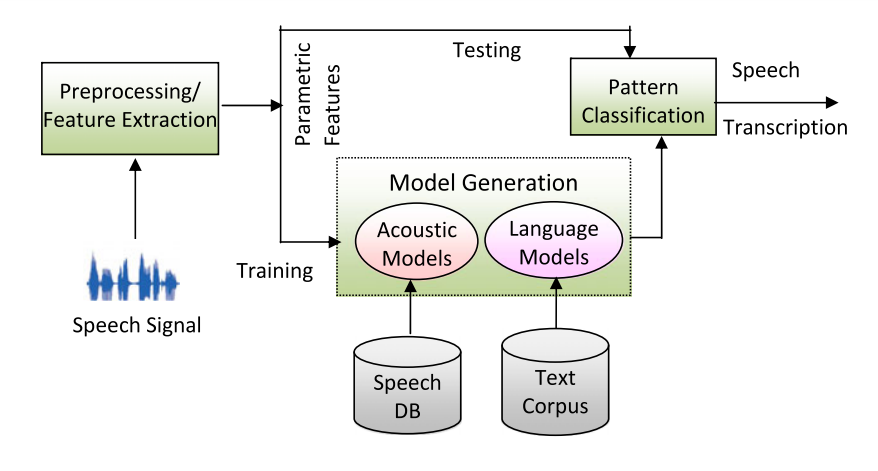
\includegraphics [width = 10cm, height= 5cm]{gambar/sr_arsitektur}}
\caption{Ilustrasi Metode \textit{Fingerprinting} \citep{aggarwal2012}}.
\label{sr_arsitektur}
\end{figure}

\section{\textit{Received Signal Strength Indicator} (RSSI)}
\textit{Received Signal Strength Indicator} atau RSSI adalah metode pengukuran jarak yang memperoleh sinyal dari transmiter seperti \textit{Bluetooth} untuk menentukan \textit{distance-loss} model, dan kemudian memperkirakan posisi pengguna melalui beberapa algoritma (\citep{li2018indoor}). Menurut \citep{puspitasari2020} \textit{Positioning System} menghasilkan data yang penting untuk menghitung lokasi pengguna. \textit{Time of Arrival} (TOA), \textit{Time Difference of Arrival} (TDOA), \textit{Angle of Arrival} (AOA). RSSI memperkirakan jarak \textit{node} yang belum diketahui ke referensi \textit{node} dari beberapa kumpulan unit perhitungan dengan menggunakan atenuasi kekuatan sinyal (\textit{signal strength}) yang dipancarkan oleh transmiter \citep{puspitasari2020}.

\par Nilai RSSI didefinisikan dengan bilangan negatif. Semakin tinggi bilangan negatifnya, maka kekuatan sinyal tersebut tergolong lemah. Namun apabila nilainya mendekati 0, maka sinyal tersebut tergolong kuat. RSSI dapat digolongkan menjadi 5 kategori kekuatan sinyal seperti pada \ref{tab:sinyal_rssi}

\begin{table}[]
\caption{Kekuatan sinyal RSSI \citep{sideeq2016smart}}
\label{tab:sinyal_rssi}
\begin{tabular}{|l|l|l|}
\hline
{\color[HTML]{000000} \textbf{No.}} & \textit{\textbf{Signal Noise Ratio }}(SNR) & \textbf{RSSI} \\ \hline
1. & Kurang dari -40 dB   & Luar Biasa  \\ \hline
2. & -40 dB hingga -55 dB & Sangat Baik \\ \hline
3. & -55 dB hingga -70 dB & Baik        \\ \hline
4. & -70 dB hingga -80 dB & Cukup Baik  \\ \hline
5. & Lebih dari -80 dB    & Buruk       \\ \hline
\end{tabular}
\end{table}

\section{\textit{Bluetooth Low Energy)} (BLE)}
Teknologi \textit{Bluetooth} dikembangkan oleh Ericsson pada tahun 1994 dengan kegunaan sebagai standar komunikasi nirkabel untuk bertukar data dalam jarak dekat \citep{kaluvza2017analysis}. Teknologi \textit{Bluetooth} memiliki fitur utama yaitu memiliki biaya yang rendah, konsumsi daya rendah, jangkauan kecil, memiliki ketahanan dan penggunaan secara global. Kecepatan transfer data yang diberikan oleh \textit{Bluetooth} sebesar 1 Mbit/s dan menggunakan pita frekuensi tanpa izin 2,4 hingga 2,485 GHz \citep{kaluvza2017analysis}.

\par Pertengahan tahun 2010 spesial otoritas kompeten yang bernama “Bluetooth Special Interest Group" (SIG) mengumumkan spesifikasi \textit{Bluetooth} 4.0, dimana meliputi : \textit{Bluetooth} Klasik, \textit{Bluetooth} dengan kecepatan tinggi, dan protokol \textit{Bluetooth} hemat energi. Karakteristik dari \textit{Bluetooth Low Energy} (BLE) adalah memiliki ukuran yang kecil, menggunakan biaya rendah, konsumsi penggunaan daya yang rendah dengan kemungkinan penggunaan sampai beberapa tahun bekerja dengan menggunakan baterai AAA dan memiliki kompatibilitas dengan perangkat seluler, tablet, dan komputer \citep{kaluvza2017analysis}.



\section{\textit{Beacon}}
BLE memancarkan sinyal dari alat transmiter yang beroperasi menggunakan baterai. Alat transmiter tersebut disebut dengan \textit{Beacon}. \textit{Beacon} merupakan alat pendeteksi lokasi dengan harga yang terjangkau, ukurannya yang kecil, memiliki daya tahan baterai yang cukup lama, dan tidak membutuhkan energi listrik tambahan \citep{puspitasari2020}. Setiap perangkat \textit{smartphone} dan tablet yang mendeteksi sinyal dari \textit{Beacon}, dapat menghitung jarak dan memperkirakan keberadaan lokasi setiap perangkat sekaligus. \textit{Beacon Bluetooth} mengubah pengalaman menggunakan \textit{smartphone} untuk bepergian, berbelanja, bekerja, dan bermain \citep{kaluvza2017analysis}.

\section{\textit{Speech Recognition}}
\textit{Speech Recognition} adalah kemampuan suatu komputer agar dapat mengenali apa yang diucapkan oleh seseorang berdasarkan sinyal suara yang diucapkan oleh seseorang atau bisa disebut sebagai \textit{Automatic Speech Recognition} (ASR)\citep{jurafskyspeech2008}. \textit{Speech Recognition} merupakan antarmuka alami untuk berkomunikasi dengan peralatan komputer seperti \textit{smart home appliances}, \textit{personal assistants}, atau \textit{smartphone}. ASR Juga berguna untuk \textit{general transcription}, contohnya untuk membuat \textit{captions} secara otomatis untuk audio atau video (mentranskripsikan film atau video atau \textit{live discussions}) (Daniel & James, 2020). Menjadi suatu kemudahan bagi manusia jika komputer dapat memahami apa yang diucapkan oleh manusia dan karena hal itu juga manusia dapat dengan mudah mengoperasikan komputer karena adanya teknologi yang \textit{Automatic Speech Recognition}. serta \textit{speech synthesis} atau \textit{text-to-speech} (TTS) \citep{jurafskyspeech2008}.

\section{\textit{Text-to-Speech }(TTS)}
Speech Syntesis atau text-to-speech merupakan kebalikan dari ASR dalam memetakan teks ke bentuk gelombang akustik. TTS memilik berbagai macam aplikasi. TTS digunakan dalam agen percakapan yang berdialog dengan orang-orang, berperan dalam perangkat yang membacakan dengan keras untuk tunanetra atau dalam permainan, dan dapat digunakan untuk berbicara bagi penderita gangguan neurologis, seperti mendiang Steven Hawking seorang ahli astrofisika berbicara dengan memanipulasi sistem TTS \citep{jurafskyspeech2008}.

\section{KALDI \textit{Toolkit}}
Kaldi adalah toolkit open-source untuk speech recognition, Kaldi ditulis dalam bahasa C++ dan di bawah lisensi Apache v2.0, Kaldi bergantung dengan library finite-state transducers (menggunakan OpenFst) serta library aljabar linier ekstensif menggunakan "Basic Linear Algebra Subroutines" (BLAS) dan "Linear Algebra PACKage" (LAPACK) \citep{povey2011}. Pada penelitian ini akan digunakan model yang dihasilkan oleh Kaldi untuk membangun model yang akan digunakan pada VOSK API.


\section{VOSK API}
Vosk api merupakan toolkit untuk speech recognition, di mana memiliki beberapa kelebihan, yaitu \citep{cephei2019}:
\begin{enumerate}
\item Memiliki 19 lebih bahasa dan dialek yang didukung vosk.
\item Vosk api merupakan toolkit speech recognition yang bisa digunakan secara offline, yang dapat digunakan pada Raspberry Pi, Android, iOS.
\item Kemudahan untuk menginstalasi vosk dengan menggunakan pip3 install vosk.
\item Model yang portabel pada masing-masing bahasa sebesar 50Mb, namun ada beberapa model server yang lebih besar pula.
\item Menyediakan streaming API untuk pengalaman pengguna terbaik.
\item Memiliki beberapa paket bahasa pemograman yang berbeda-beda, seperti java, csharp, javascript dll.
\item Untuk akurasi terbaik dapat memungkinkan konfigurasi ulang kosakata dengan cepat.
\item Mendukung identifikasi pembicara selain dengan speech recognition yang sederhana.

\end{enumerate}

\section{Android}
Android merupakan suatu \textit{software} (perangkat lunak) yang digunakan pada \textit{mobile device}(perangkat berjalan)yang meliputi sistem operasi, \textit{middleware},dan aplikasi inti. Android \textit{Standart Development Kit} (SDK) menyediakan alat dan \textit{Application Programming Interface}(API) yang diperlukan untuk memulai pengembangan aplikasi pada platform Android menggunakan bahasa pemrograman Java, yaitu kode Java yang terkompilasi dengan data dan \textit{file resources} yang dibutuhkan aplikasi dan digabungkan oleh \textit{app tools} menjadi paket Android. \textit{File} tersebut ditandai dengan ekstensi .apk. \textit{File} inilah yang didistribusikan sebagai aplikasi dan dipasang pada perangkat \textit{mobile} \citep{nasution2018perancangan}.

\par Menurut \citep{shaheen2017android}. Ada 4 jenis komponen aplikasi. Setiap jenis memiliki tujuan yang berbeda dan memiliki siklus proses yang berbeda yang menentukan bagaimana komponen di \textit{create} dan di \textit{destroy}. Berikut adalah ke 4 jenis komponen tersebut:

\begin{enumerate}
\item \textit{Activities}, merupakan sebuah \textit{activity} merepresentasikan tampilan aplikasi kepada pengguna (\textit{user interface}).
\item \textit{Service}, merupakan komponen yang berjalan pada \textit{background} untuk menjalankan operasi atau proses yang tidak memiliki \textit{user interface}.
\item \textit{Content Providers}, merupakan komponen yang menangani data antar aplikasi.
\item \textit{Broadcast Receivers}, merupakan komponen yang bertanggung jawab atas menerima serta menyampaikan informasi atau notifikasi.
\end{enumerate}

\section{Android Studio}
Android Studio merupakan \textit{Integrated Development Environtment} (IDE) untuk pengembangan platform Android. Android Studio diumumkan pada tanggal 16 Mei 2013 di Google I/O \textit{Conference}. Android Studio dapat digunakan secara gratis di bawah pengawasan Apache \textit{License} 2.0. Android Studio merupakan kolaborasi antara JetBrains dan Google. Android Studio mirip dengan Eclipse yang disertai dengan ADT \textit{Plugin} (Android \textit{Development Tools})\citep{craig2015learn}.

\par Fitur-fitur Android Studio menurut \citep{puspitasari2020} adalah sebagian berikut:
\begin{itemize}
\item Proyek berbasis pada Gradle \textit{Build}.
\item \textit{Refactory} dan perbaikan bug yang cepat.
\item \textit{Tools} baru yang bernama "Lint" diklaim dapat memonitor kecepatan, kegunaan, serta kompatibilitas aplikasi dengan cepat.
\item Mendukung Proguard and \textit{App-signing} untuk keamanan.
\item Memiliki GUI aplikasi Android lebih mudah.
\item Didukung oleh Google \textit{Cloud Platform}, sehingga lebih mudah mengintegrasi Google \textit{Cloud Messaging and Application Engine} untuk setiap aplikasi yang dikembangkan.
\end{itemize}

\section{SCRUM}
\textit{Scrum} adalah \textit{development framework} di mana tim lintas-fungsi mengembangkan produk atau proyek secara berulang dan bertahap. \textit{Scrum} menyusun siklus pengembangan yang disebut \textit{Sprint}. Iterasi ini masing-masing tidak lebih dari empat minggu dan berlangsung satu demi satu tanpa jeda \citep{deemer2012lightweight}. \textit{Sprint} memiliki durasi tetap atau \textit{Sprint} berakhir pada tanggal tertentu baik selesai atau belum, dan tidak pernah diperpanjang. Oleh karena itu \textit{Sprint} dikatakan \textit{timeboxed} \citep{schwaber2011scrum}. Tahapan-tahapan metode \textit{Scrum} menurut \citep{schwaber2011scrum} adalah sebagai berikut :

\begin{enumerate}
\item Dimulai dengan mengumpulkan \textit{user requirements}, namun tidak harus semua \textit{requirements} diharapkan harus keluar dari pemikiran pengguna di tahap awal proses pengembangan. Pengguna dapat mengubah pikiran mereka di setiap waktu selama proses pengembangan, pengguna dapat menambah fitur-fitur baru, menghapus atau memperbaharui beberapa fitur yang telah ada sebelumnya.

\item Tahapan selanjutnya adalah memprioritaskan \textit{requirements} dan \textit{Product Backlog}. Sebuah perencanaan yang tepat dalam \textit{Sprint} harus dilakukan sesuai dengan jumlah Sprint yang dibutuhkan untuk mengembangkan perangkat lunak, yang terdiri dari durasi \textit{Sprint} tersebut dan \textit{requirements} apa saja yang terdapat di \textit{Product Backlog} yang harus diimplementasikan di setiap \textit{Sprint} (dikenal dengan \textit{Sprint Backlog}).

\item \textit{Sprint} diawali dengan \textit{Sprint Planning} di mana \textit{Product Owner}, satu orang uang telah diberikan wewenang dan bertanggung jawab untuk memaksimalkan nilai produk di pasar, bertemu dengan tim \textit{Scrum} (tim dengan jumlah 2-9 orang), kemudian bekerja sama untuk memperkirakan \textit{requirements} dari \textit{Product Backlog} apa saja yang dikerjakan selama satu \textit{Sprint}.

\item \textit{Sprint Planning} difasilitasi dengan \textit{Scrum Master}. \textit{Scrum Master} adalah seorang pemimpin yang melayani (\textit{Servant Leader}). \textit{Sprint Planning} memiliki batasan waktu selama 8 jam di dalam sebuah \textit{Sprint} yang berdurasi selama 30 hari. Keluaran dari \textit{Sprint Planning} adalah daftar pekerjaan dari hasil kesepakatan antara \textit{Product Owner} dan tim \textit{Scrum} di mana pekerjaan itu yang dikerjakan oleh tim \textit{Scrum} nantinya selama satu \textit{Sprint} beserta \textit{Sprint Goal} yang dinamakan dengan \textit{Sprint Backlog}.

\item Setelah \textit{Sprint Planning} berakhir, tim \textit{Scrum} akan mengambil \textit{Sprint Backlog} untuk diri mereka masing-masing dan mengerjakan \textit{Sprint Backlog} setiap hari hingga akhir \textit{Sprint} tanpa campur tangan dari pihak mana pun. \textit{Daily Scrum} akan dikerjakan oleh tim \textit{Scrum} yang tidak lebih dari 15 menit untuk menentukan apa saja yang akan mereka kerjakan selama 24 jam ke depan berdasarkan perkembangan 24 jam terakhir, serta menyampaikan permasalahan yang menghambat mereka untuk bisa mencapai \textit{Sprint Goal}. Tim \textit{Scrum} akan melakukan perbaikan-perbaikan item dari \textit{Product Backlog} pada \textit{Sprint} yang akan datang selama proses pengembangan berlangsung, dengan tujuan membuat \textit{Sprint Planning} menjadi lebih efektif.

\item Di akhir Sprint saat acara \textit{Sprint Review}, \textit{Product Owner} akan mempresentasikan hasil pekerjaan tim \textit{Scrum} selama satu \textit{Sprint} dan juga menjelaskan apa saja pencapaian tim \textit{Scrum} menuju \textit{Sprint Goal} di dalam \textit{Sprint} tersebut kepada para pemegang kepentingan (\textit{stakeholder}) agar mendapatkan \textit{feedback}. \textit{Feedback} ini akan dimasukkan ke dalam \textit{Product Backlog} agar meningkatkan nilai dari sebuah produk. \textit{Sprint Review} memiliki batasan waktu tidak lebih dari 4 jam untuk \textit{sprint} yang memiliki durasi selama 30 hari.

\item Setelah \textit{Sprint Review}, \textit{Scrum Master} memfasilitasi acara yang bernama \textit{Sprint Retrospectives} agar tim \textit{Scrum}, \textit{Product Owner} bekerja sama menentukan apa saja peningkatan yang akan mereka implementasikan di \textit{Sprint} berikutnya. \textit{Definition of Done} adalah salah satu hal yang ditekankan oleh tim \textit{Scrum} pada saat \textit{Sprint Retrospectives}.

\item \textit{Sprint Retrospectives} merupakan acara yang paling penting dalam \textit{Scrum} dikarenakan sifatnya yang menekankan \textit{continuous learning} yang dapat meningkatkan tingkat \textit{agility} perusahaan. \textit{Sprint Review} memiliki batasan waktu tidak lebih dari 3 jam untuk \textit{Sprint} yang memiliki durasi selama 30 hari. Setelah \textit{Sprint Retrospectives} berakhir, maka \textit{Sprint} berikutnya akan langsung dilakukan tanpa jeda antar \textit{Sprint}. Pada setiap \textit{Sprint}, \textit{Product Owner} akan memastikan agar produk mencapai nilai setinggi mungkin saat pengembangan produk diakhiri. \textit{Product Owner}, \textit{Scrum Master} dan tim \textit{Scrum} memegang komitmen, keberanian, saling menghargai satu sama lain, keterbukaan dan fokus. Ilustrasi tahapan-tahapan metode \textit{Scrum} dapat dilihat pada \ref{img:scrum} di bawah ini.
\end{enumerate}

\begin{figure}[H]
\centering
\shadowbox
{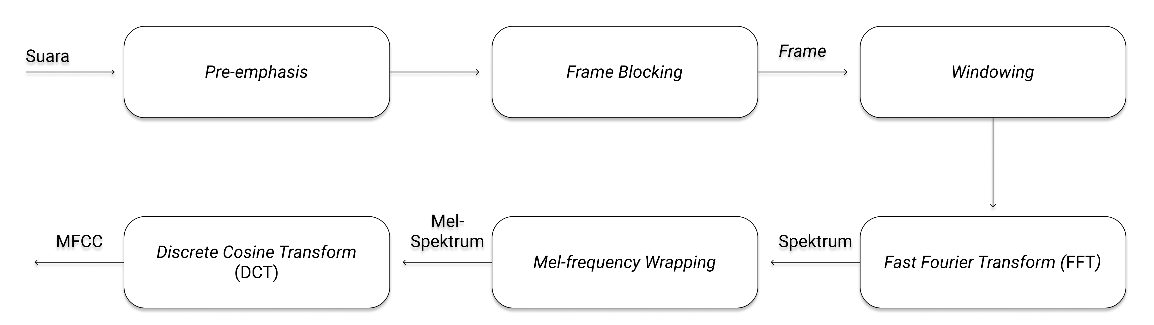
\includegraphics [width = 14cm, height= 5cm]{gambar/alir_mfcc}}
\caption{Ilustrasi Metode Pengembangan Menggunakan Scrum \citep{schwaber2011scrum}.}}.
\label{img:scrum}
\end{figure}

\section{\textit{Black Box Testing}}
Salah satu jenis pengujian fungsional adalah \textit{blackbox testing}. \textit{Blackbox} testing merupakan suatu pengujian yang tidak menggunakan pengetahuan tentang struktur interior aplikasi. Saat melakukan pengujian, penguji akan berinteraksi langsung dengan \textit{user interface}, lalu penguji akan memberikan masukan dan memeriksa hasil dari aplikasi yang digunakan tanpa mengetahui bagaimana proses dari hasil tersebut \citep{xu2016comparative}. Pada \textit{blackbox testing} mendapatkan pengujian dari deskripsi eksternal perangkat lunak, termasuk spesifikasi, persyaratan, dan desain \citep{ammann2016introduction}.

\par \textit{Blackbox testing} memiliki beberapa keuntungan, di antaranya penguji tidak perlu mengetahui suatu bahasa pemrograman, pengujian dilakukan dari sudut pandang pengguna agar dapat mengetahui suatu inkonsisten pada spesifikasi kebutuhan serta yang terakhir programmer dan penguji dapat saling bergantung \citep{jaya2018pengujian}. \textit{Blackbox testing} juga memiliki beberapa kekurangan yaitu suatu pengujian sulit didesain tanpa spesifikasi yang jelas, memiliki kemungkinan untuk pengulangan \textit{testing} dan tidak ada pengujian pada bagian \textit{back-end} \citep{jaya2018pengujian}.

\section{\textit{Usability Testing}}
\textit{Usability Testing} adalah kegiatan pengujian untuk mengumpulkan data mengenai sebuah produk dalam tahap pengembangan. Tujuan utama dari \textit{usability testing} adalah untuk mengumpulkan data kuantitatif dengan mengukur waktu untuk mengidentifikasi dan memperbaiki kekurangan yang ada dalam produk serta bahan pendukung yang menyertainya sebelum produk dirilis \citep{rubin2008handbook}. Dengan \textit{usability testing}, didapati apa yang sebenarnya dilakukan pengguna, apa yang berhasil untuk mereka, dan apa yang tidak dipikirkan akan mereka lakukan atau bahkan apa yang mereka pikir akan mereka lakukan jika menggunakan produk \citep{barnum2020usability}.


\par Pengujian ini diharapkan akan mendapatkan kekuatan dan kelemahan dari setiap aspek yang ada pada aplikasi itu sendiri. Maka dari itu, perlu adanya dokumentasi pengalaman aktual para calon pengguna aplikasi atau produk saat dievaluasi \citep{wesfix2017branding}. Tujuan lain dilakukannya pengujian ini adalah untuk mengumpilkan data kualitatif yang berhubungan dengan produk yang diuji. Data kualitatif tersebut terdiri dari komentar yang dibuat oleh partisipan, jawaban dari kuesioner pertanyaan dan tanggapan dari partisipan saat proses wawancara. \textit{Usability testing} telah terbukti dapat mengurangi waktu pada tahap pengembangan, mengurangi jumlah bugs, dan menghasilkan produk yang lebih berkualitas untuk meningkatkan nilai jual \citep{wahl2000student}.


\section{\textit{System Usability Scale }(SUS)}
Kuesioner standar yang paling sering digunakan untuk penilaian suatu kegunaan merupakan \textit{System Usability Scale} (SUS). Dari awal kuesioner ini relatif tidak menguntungkan, namun dimasa depan kemungkinan besar SUS akan menjadi suatu ukuran yang populer dari persepsi kegunaan. Mendapatkan nilai pada SUS cukup rumit, karena pola pada \textit{item} yang bergantian dan memiliki keputusan awal untuk memanipulasi skor berada di antara 0 sampai 100 \citep{lewis2018system}. John Brooke mengembangkan SUS pada tahun 1996 yang berisi 10 pertanyaan dasar dan sederhana tentang kegunaan suatu sistem, berikut adalah pertanyaannya \citep{kaya2019usability}:

\begin{center}
\begin{tabular}{ |c|c| } 
 \hline
 R1 & Saya pikir saya ingin menggunakan sistem ini dengan sering.\\
 R2 & Saya menemukan sistem yang tidak rumit.\\
 R3 & Saya pikir sistemnya mudah digunakan.\\
 R4 & Saya pikir saya akan membutuhkan bantuan dari orang teknis untuk dapat menggunakan sistem ini.\\
 R5 & Saya menemukan berbagai fungsi dalam sistem ini terintegrasi dengan baik.\\
 R6 & Saya pikir ada terlalu banyak inkonsistensi dalam sistem ini.\\
 R7 & Saya membayangkan bahwa kebanyakan orang akan belajar menggunakan sistem ini dengan sangat cepat.\\
 R8 & Menurut saya sistem ini sangat rumit untuk digunakan.\\
 R9 & Saya merasa sangat percaya diri menggunakan sistem ini.\\
 R10 & Saya perlu belajar banyak hal sebelum saya bisa menggunakan sistem ini.\\
 \hline
\end{tabular}
\end{center}

\par Pertanyaan tersebut akan diberikan kepada peserta uji dan menjawab dengan skala antara 1 (Sangat tidak setuju) dan 5 (Sangat setuju). Menurut Brooke hasil dari jawaban akan dievaluasi dalam kisaran 0 sampai 4. Dapat dilihat pada pertanyaan yang memiliki nomor ganjil maka memiliki makna positif dan pertanyaan bernomor genap memiliki makna negatif. Pada pertanyaan positif dilakukan penilaian yang mana skor pengguna dikurangi 1 poin dan pada pertanyaan negatif dilakukan penilaian yang mana skor pengguna dikurangi 5 poin. Setelah itu jumlah skor yang didapat dikalikan 2,5 untuk membuat kisaran antar 0 sampai 100. Skor SUS rata-rata dan skala peringkat kata sifat dihitung untuk setiap aplikasi seluler di Android dan iOS \citep{kaya2019usability}.


%-----------------------------------------------------------------------------%

% Baris ini digunakan untuk membantu dalam melakukan sitasi
% Karena diapit dengan comment, maka baris ini akan diabaikan
% oleh compiler LaTeX.
\begin{comment}
\bibliography{daftar-pustaka}
\end{comment}


%-------------------------------------------------------------------------------
%                            BAB III
%               		METODOLOGI PENELITIAN
%-------------------------------------------------------------------------------
\fancyhf{} 
\fancyfoot[C]{\thepage}
\chapter{METODOLOGI PENELITIAN}

\section{Waktu dan Lokasi Penelitian}
Penelitian ini akan bertempat pada Gedung A Fakultas Matematika dan Ilmu Pengetahuan Alam. Waktu yang dibutuhkan agar penelitian ini dapat diimplementasikan adalah 6 bulan terhitung dari Oktober 2022 hingga Maret 2023.

\section{Alat dan Bahan}
Alat dan Bahan yang akan digunakan pada penelitian ini terdiri dari beberapa perangkat keras (\textit{Hardware}) dan perangkat lunak (\textit{Software}) yang dijabarkan sebagai berikut:

\begin{enumerate}
\item Perangkat Keras
	\begin{itemize}
	\item Laptop Acer Aspire E5-475g dengan RAM 16GB, Intel Core i5-7200U 2.5GHz, Nvidia GeForce 940MX 2GB, \textit{Harddisk} (HDD) 1500Gb, \textit{Solid State Drive} (SSD) 250GB.
	\item \textit{Smartphone} Xiaomi Poco F3 dengan RAM 6GB, \textit{Internal Storage} 128GB.
	\item \textit{Personal Computer} dengan AMD Ryzen 7 2700x, RAM 16GB, Nvidia GeForce RTX 2080 8GB, \textit{Solid State Drive} (SSD) 500GB.
	\item \textit{Beacon Bluetooth}.
	\end{itemize}

\item Perangkat Lunak
	\begin{itemize}
	\item Windows 11 Pro
	\item Linux Ubuntu 20.04.1 LTS
	\item Android Studio 2021.2.1.15
	\item Visual Studio Code
	\item Figma
	\item Notion
	\item Vosk API
	
	\end{itemize}
\end{enumerate}


\newpage
\section{\textit{Roadmap} Penelitian}
\textit{Roadmap} penelitian merupakan diagram yang menggambarkan rangkaian beberapa penelitian yang saling berkesinambungan dalam rentang waktu tertentu. \textit{Roadmap} penelitian biasa dibuat untuk memberikan batasan kepada peneliti agar menghindari pengamatan yang tidak perlu dan fokus terhadap bagian penelitiannya saja. Pada penelitian ini dibagi ke dalam 2 fase. Fase pertama pada tahun 2019 memiliki fokus penelitian pada \textit{indoor localization} dengan menggunakan \textit{Bluetooth Low Energy} (BLE) dan menggunakan \textit{Wireless Local Area Network} (WLAN) dapat dilihat gambar \ref{img:fase1}. Pada fase kedua pada tahun 2020 lebih berfokus pada penelitian \textit{Indoor Localization} dengan menggunakan BLE. Penelitian ini terletak pada fase 2 di tahun 2020 dengan topik utama yaitu Aplikasi Navigasi \textit{Indoor} dengan sub topik untuk pengguna Tunanetra. Penelitian ini memiliki batasan berupa pembangunan aplikasi \textit{mobile} untuk \textit{Route Guidance} untuk Tunanetra, seperti yang ditunjukkan pada gambar \ref{img:fase2} dengan kata yang dicetak tebal berwarna merah sebagai berikut.


\begin{figure}[H]
  \begin{adjustbox}{addcode={\begin{minipage}{\width}}{\caption{%
      \textit{Roadmap} Penelitian Fase 1
      }\label{img:fase1}\end{minipage}},rotate=90,center} %label gambar simpen disetelah capt
      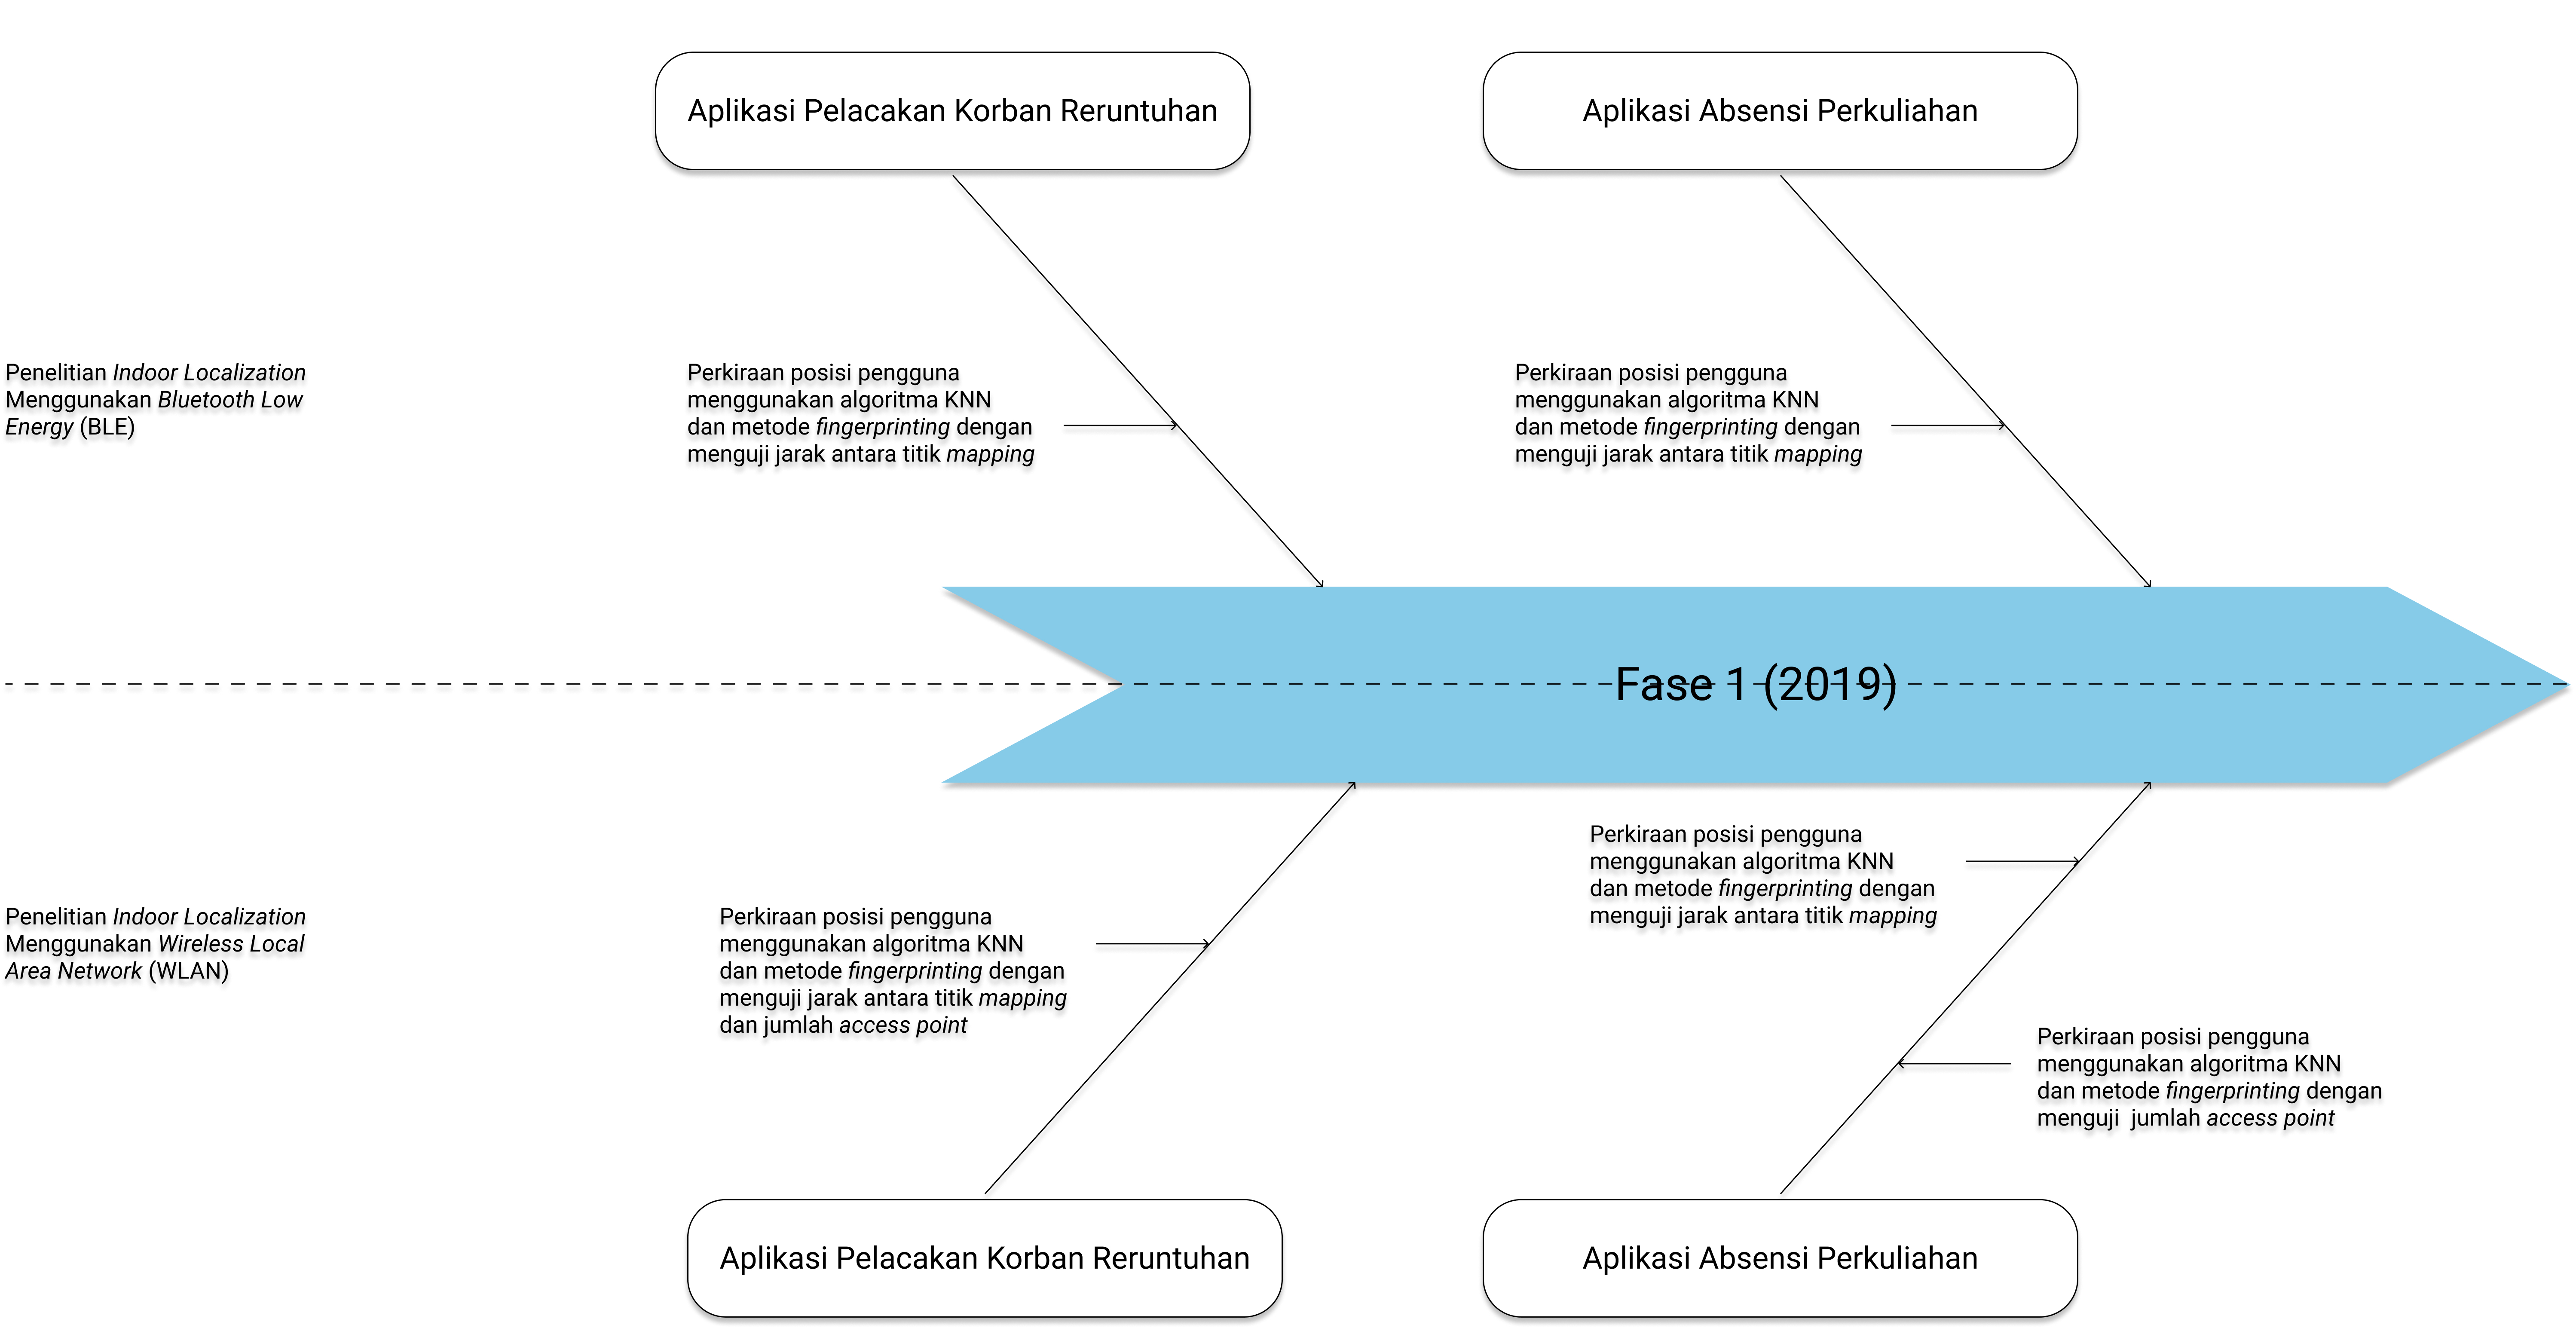
\includegraphics[scale=.3]{gambar/bab3/rp_fase1}%
  \end{adjustbox}
\end{figure}

\fancyhf{} 
\fancyfoot[R]{\thepage}

\begin{figure}[H]
  \begin{adjustbox}{addcode={\begin{minipage}{\width}}{\caption{%
      \textit{Roadmap} Penelitian Fase 2
      }\label{img:fase2}\end{minipage}},rotate=90,center}
      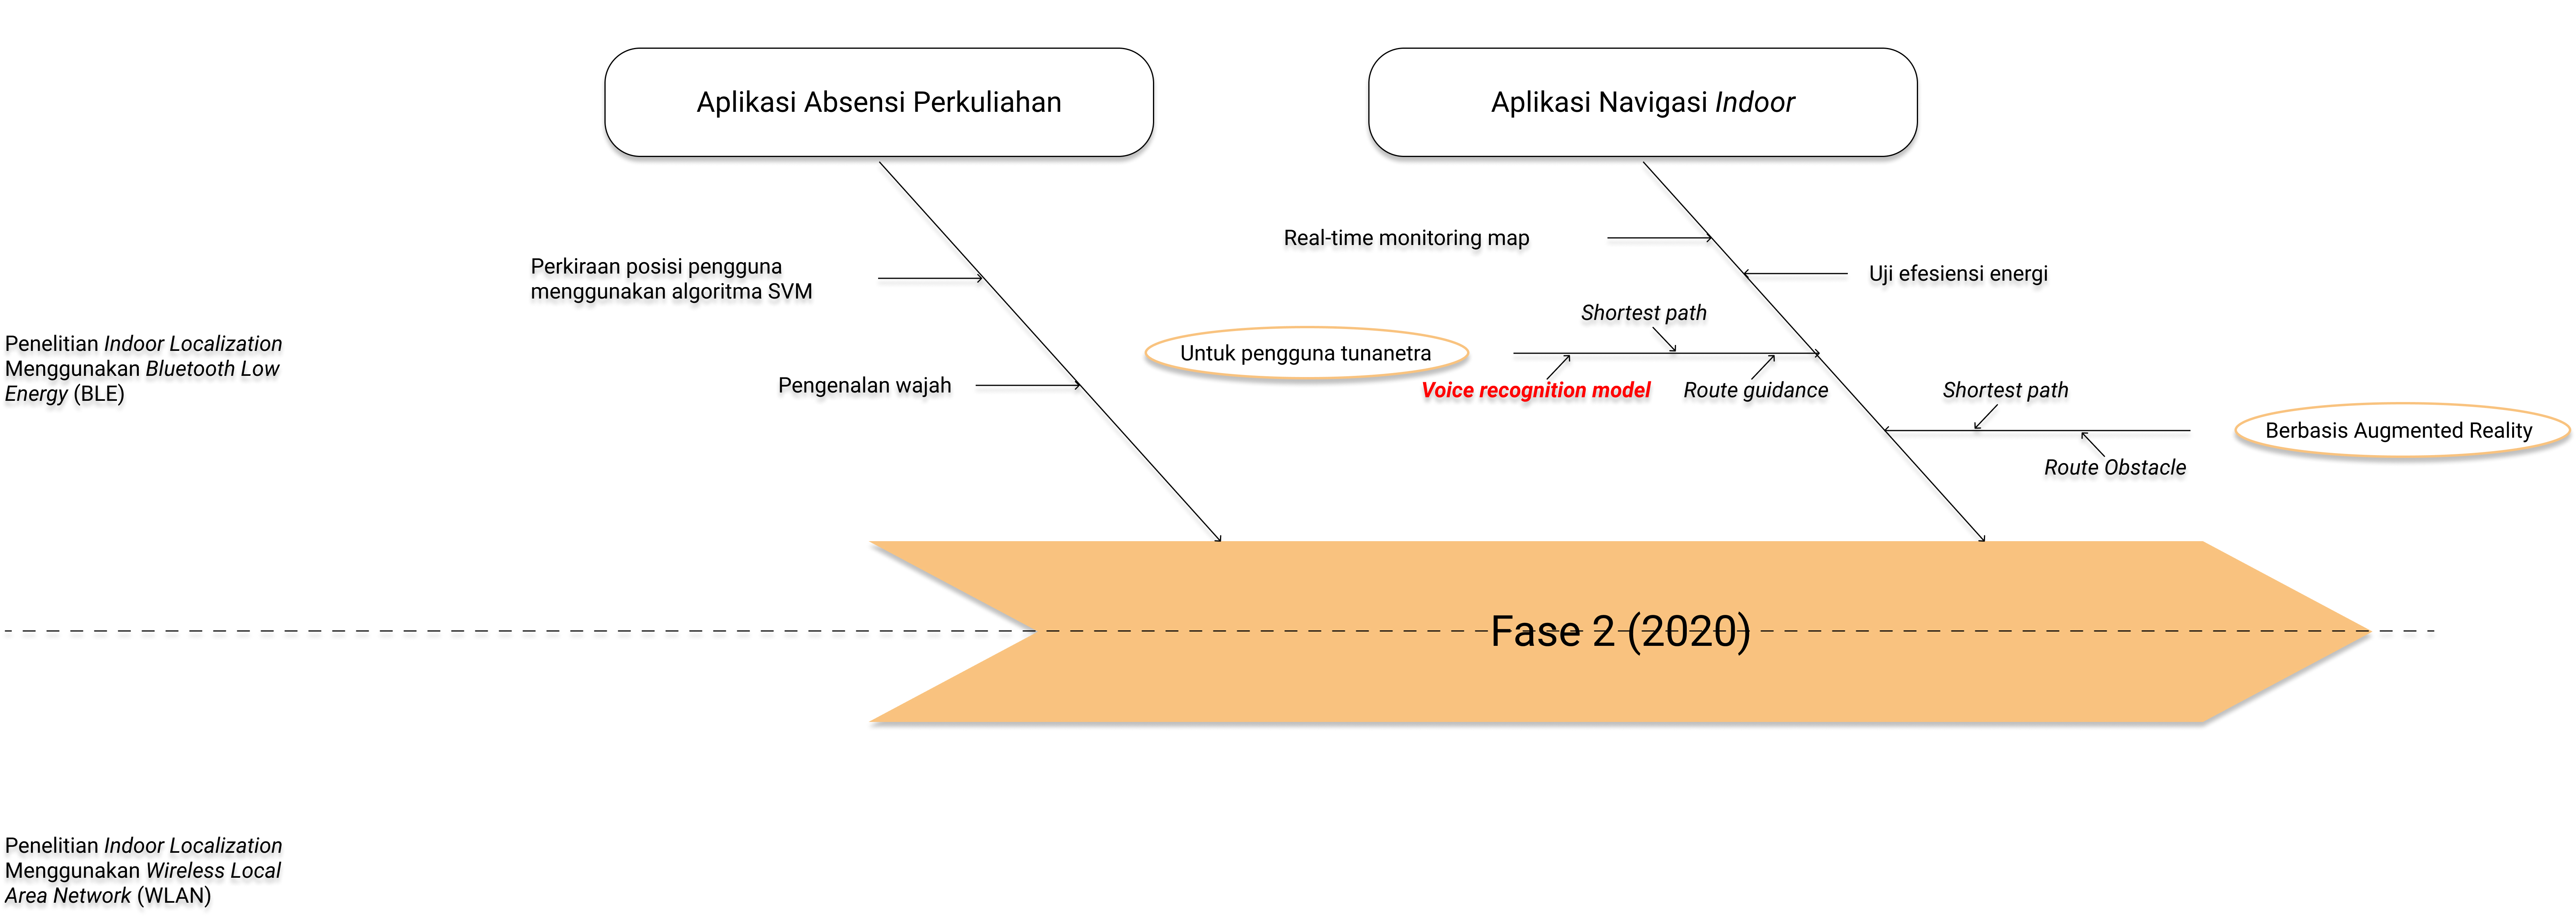
\includegraphics[scale=.6]{gambar/bab3/rp_fase2}%
  \end{adjustbox}
\end{figure}

\fancyhf{} 
\fancyfoot[R]{\thepage}

\section{Metode Penelitian}
Metode penelitian yang dilakukan dalam penelitian ini ditunjukkan pada Gambar \ref{img:diagram_alir_penelitian}.

\begin{figure}[H]
\centering
{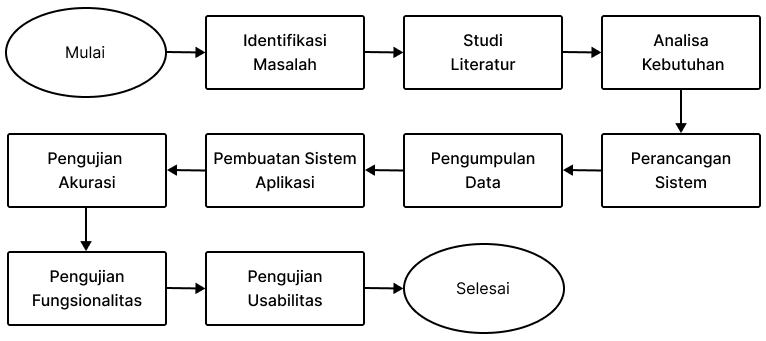
\includegraphics [scale= 0.6]{gambar/bab3/diagram_alir}}
\caption{Diagram Alir Penelitian}
\label{img:diagram_alir_penelitian}
\end{figure}

\fancyhf{} 
\fancyfoot[R]{\thepage}

\newpage
\subsection{Identifikasi Masalah}
Tahapan ini merupakan tahapan yang dilakukan untuk mengidentifikasi masalah pada lingkungan yang berhubungan dengan aplikasi yang akan dibuat baik secara langsung maupun tidak langsung dan menjadi landasan mengapa aplikasi ini harus dibuat. Masalah-masalah yang berhasil di identifikasi adalah sebagai berikut:

\begin{itemize}
\item Belum ada teknologi \textit{Route Guidance System/Wayfinding System} berbasis \textit{Indoor positioning} dengan panduan rute menggunakan \textit{Speech Command Recognition} di Universitas Syiah Kuala.

\item Membantu Tunanentra menemukan ruangan di Gedung A FMIPA Universitas Syiah Kuala dipandu dengan navigasi suara.

\end{itemize}



%%%%%%%%%%%%%%%%%%%%%%%%%%%%%%%%%%%%%%%%%%%
\subsection{Studi Literatur}
Studi literatur digunakan sebagai bahan referensi selama proses penelitian. Studi literatur dilakukan dengan cara mencari situs \textit{website} dan jurnal-jurnal terkait tentang penelitian, baik jurnal nasional maupun internasional, buku-buku yang telah diterbitkan, serta situs-situs internet yang berkaitan dengan permasalahan yang dikaji dalam penelitian. Studi literatur dapat dikembangkan untuk menyempurnakan kekurangan dari penelitian sebelumnya.

%%%%%%%%%%%%%%%%%%%%%%%%%%%%%%%%%%%%%%%%%
\subsection{Analisa Kebutuhan}
Pada tahapan ini dilakukan proses analisa kebutuhan yang bersumber dari masalah yang di identifikasi sebelumnya. Proses pembangunan aplikasi akan didasarkan pada kebutuhan yang ada. Berikut adalah hasil analisa dari beberapa kebutuhan dari sistem yang akan dibangun.
\begin{enumerate}
\item Kebutuhan Fungsional
\par Kebutuhan fungsional mendefinisikan fungsionalitas sistem. Kebutuhan fungsional dari identifikasi masalah yang telah dilakukan adalah sebagai berikut:

\begin{itemize}
\item Melakukan proses pemanduan kepada pengguna secara \textit{background process} dengan bantuan \textit{speech command recognition} dan \textit{route guidance} dengan aplikasi berbasis Android.

\item Menampilkan prediksi lokasi pengguna serta rute terbaik menuju ke lokasi tujuan pengguna.

\end{itemize}

\newpage
\item Kebutuhan Non-Fungsional
\par Kebutuhan non-fungsional memastikan batasan eksternal yang harus dipenuhi oleh sistem. Batasan-batasan tersebut antara lain:

\begin{itemize}
\item Proses pemanggilan aplikasi dimulai dengan memanggil \textit{hotword}.

\item Proses pencatatan dan penentuan lokasi dilakukan secara berkala dalam interval yang sesingkat-singkatnya.

\item Hanya dapat melakukan proses pemanduan rute apabila \textit{Bluetooth} pada perangkat hidup dan terhubung dengan \textit{Beacon}.

\item Sistem hanya dapat mendeteksi lokasi pengguna di dalam gedung yang telah di petakan terlebih dahulu.

\end{itemize}

\end{enumerate}

%%%%%%%%%%%%%%%%%%%%%%%%%%%%%%%%%%%%%%%%%
\subsection{Perancangan Sistem}
Tahap perancangan sistem ini meliputi perancangan alur kerja sistem yang berfungsi untuk memastikan sistem yang dibangun dapat digunakan secara baik oleh pengguna. Tahap perancangan sistem ini terbagi menjadi beberapa bagian yaitu diagram Use Case , Diagram Deployment, alur kerja sistem, \textit{Flow Diagram} dan desain prototipe berdasarkan analisa kebutuhan yang telah dijabarkan. Berikut ini merupakan tahapan tersebut:



\begin{enumerate}
\newpage
\item \textit{Use Case Diagram}
\par \textit{Use Case Diagram} merupakan gambaran interaksi antara pengguna dan sistem. Pengguna dari sistem yang akan dibangun ini adalah Tunanetra dan pengunjung gedung FMIPA USK. \textit{Use Case Diagram} dari sistem ini dapat dilihat pada Gambar \ref{img:use_case_diagram}

\begin{figure}[H]
\centering
{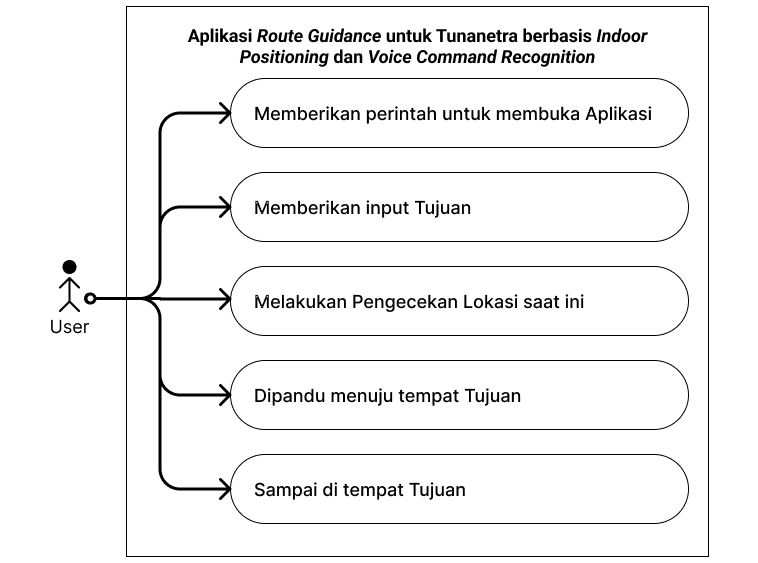
\includegraphics [width = 12cm, height= 10cm]{gambar/bab3/use_case_diagram}}
\caption{\textit{Use Case Diagram}}
\label{img:use_case_diagram}
\end{figure}


\item \textit{Deployment Diagram}
\par \textit{Deployment Diagram} merupakan gambaran hubungan antara perangkat lunak dan perangkat keras yang digunakan dalam sebuah sistem. Seperti yang telah disebutkan sebelumnya, penelitian ini merupakan bagian dari penelitian lain yang saling terintegrasi sehingga tidak semua \textit{node} dalam diagram menjadi fokus dalam penelitian ini. Bagian dalam diagram yang menjadi jangkauan dari penelitian ini ditandai dengan warna biru seperti yang ditunjukkan pada Gambar \ref{img:deployment_diagram}

\begin{figure}[H]
\centering
{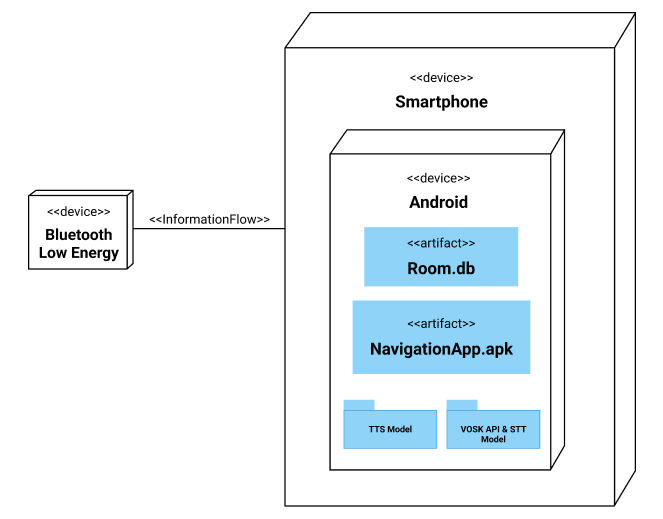
\includegraphics [width = 10cm, height= 8cm]{gambar/bab3/deployment_diagram}}
\caption{\textit{Deployment Diagram}}
\label{img:deployment_diagram}
\end{figure}


\newpage
\item Alur Kerja Sistem

\par Alur kerja sistem merupakan langkah-langkah yang dilalui sistem hingga fungsionalitas sistem dapat dimanfaatkan oleh pengguna. Alur kerja sistem ini dapat dilihat pada Gambar \ref{img:alur_kerja_sistem}

\begin{figure}[H]
\centering
{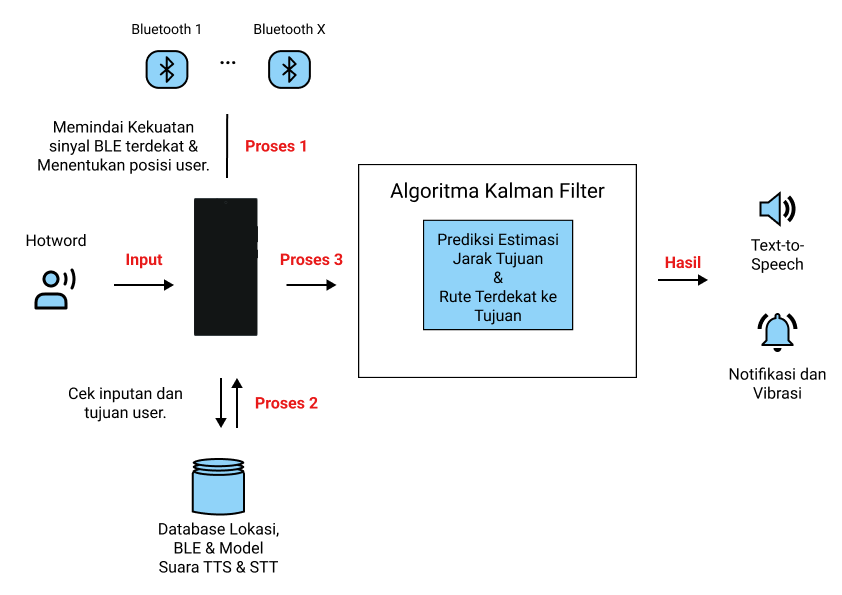
\includegraphics [scale = 0.5]{gambar/bab3/alur_kerja_sistem}}
\caption{Alur Kerja Sistem}
\label{img:alur_kerja_sistem}
\end{figure}

\begin{itemize}
\item \textit{Input} diterima dari pengguna setelah mengucapkan \textit{hotword}.

\item Pada proses 1 aplikasi dan perangkat akan memindai kekuatan sinyal BLE terdekat serta menentukan posisi pengguna.

\item Pada proses 2, setelah posisi pengguna ditentukan, aplikasi akan melakukan pengecekan \textit{input} dari pengguna pada \textit{database} lokasi menggunakan model yang telah tersedia oleh penelitian lainnya.

\item Pada proses 3, aplikasi akan memprediksi jarak tujuan serta rute terdekat menuju tujuan pengguna menggunakan algoritma Kalman Filter.

\item Hasil yang dihasilkan dari proses-proses sebelumnya berupa notifikasi dan vibrasi serta \textit{text-to-speech} atau berupa ucapan dari rute yang akan di tempuh oleh pengguna, seperti "Belok ke kanan dalam 5 langkah", "Telah sampai di tujuan , Ruangan Jurusan Informatika", dsb.
\end{itemize}

\newpage
\item \textit{Flow Diagram}
\par \textit{Flow Diagram} menunjukkan bagaimana proses tahapan melakukan navigasi pada sistem seperti pada gambar \ref{img:flow_diagram_app} berikut ini.

\begin{figure}[H]
\centering
{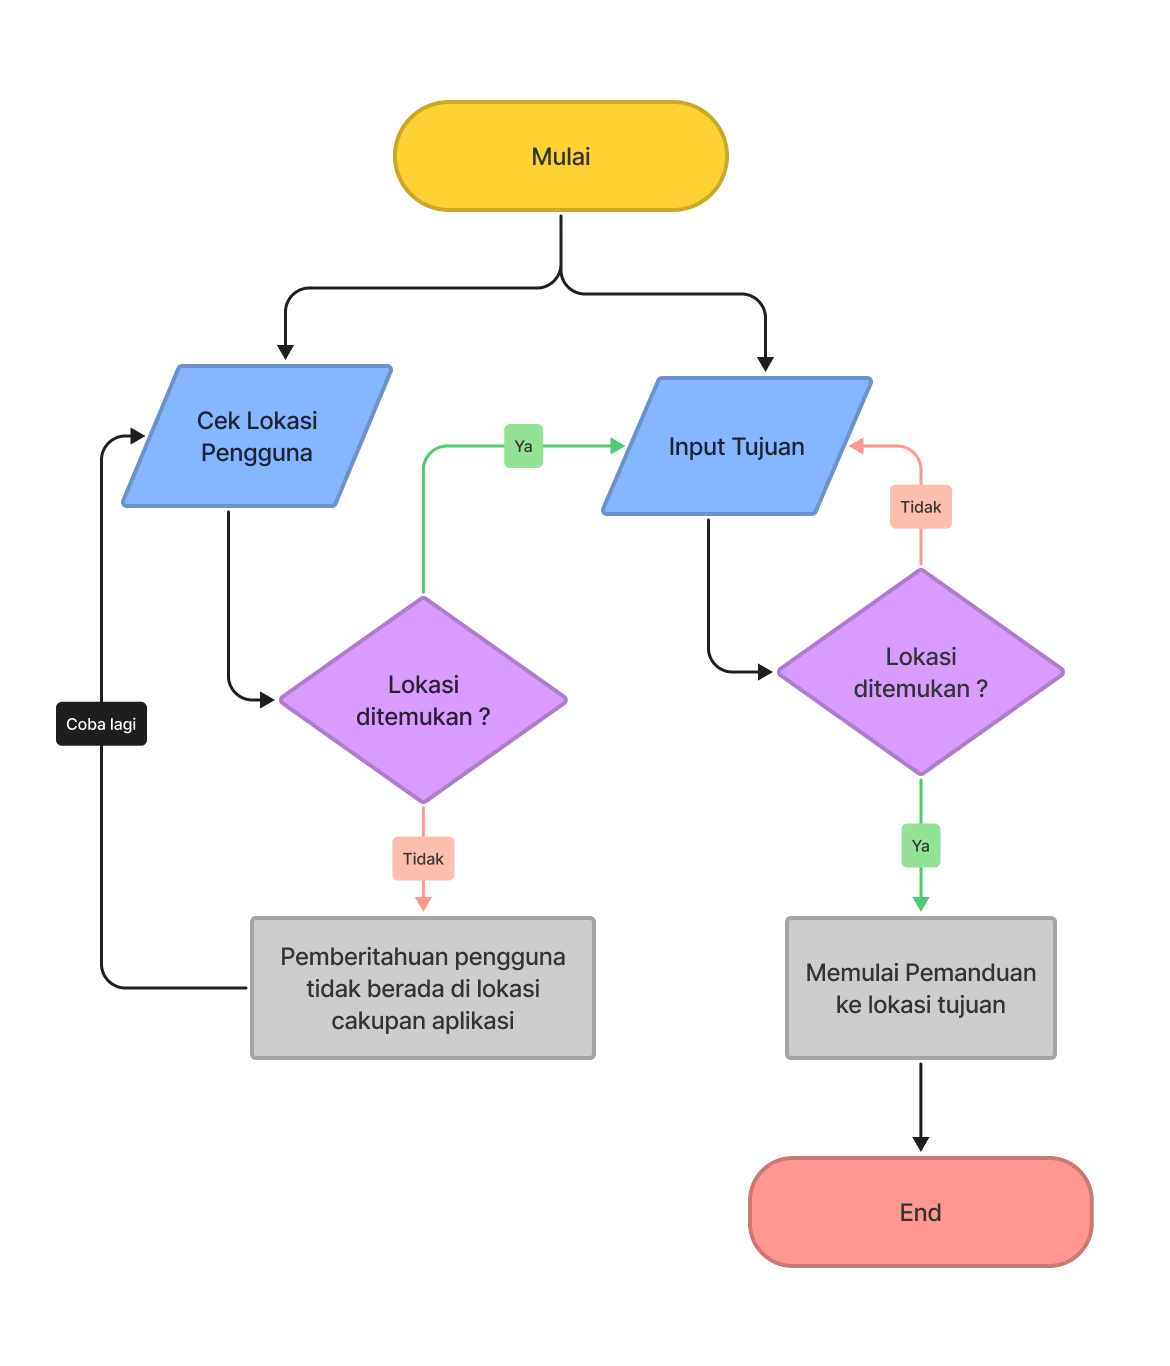
\includegraphics [scale = 0.35]{gambar/bab3/flow_diagram_app}}
\caption{\textit{Flow Diagram} Navigasi \textit{Indoor}}
\label{img:flow_diagram_app}
\end{figure}

\item Desain Prototipe
\par Desain prototipe menunjukkan perkiraan tampilan aplikasi yang akan dibuat. Desain ini dirancang berdasarkan beberapa skenario pada sisi pengguna baik tunanetra dan bukan tunanetra.

\vspace{-0cm}
	\begin{figure} [H]
	\begin{subfigure}{.5\textwidth}
  		\centering
  		% include first image
  		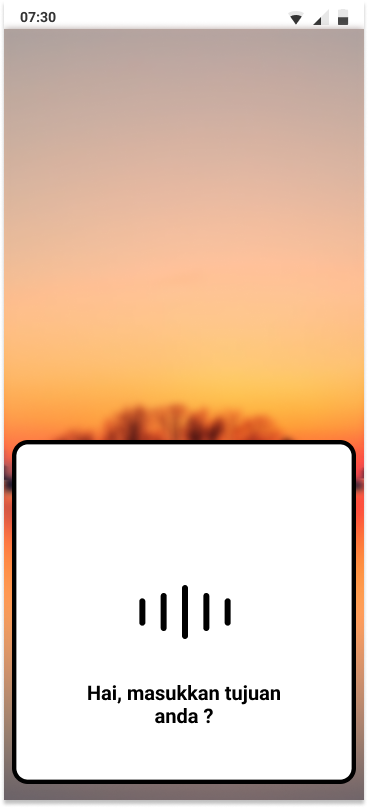
\includegraphics[width=.5\linewidth]{gambar/bab3/1}  
  		\caption{Pop up trigger by hotword}
	\end{subfigure}
	\begin{subfigure}{.5\textwidth}
  		\centering
  		% include second image
		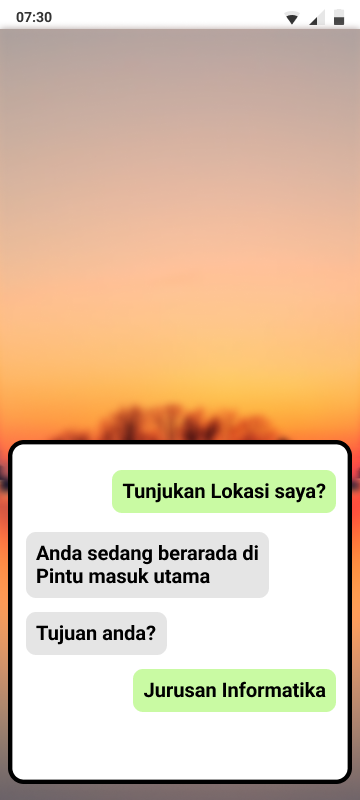
\includegraphics[width=.5\linewidth]{gambar/bab3/2}  
  		\caption{Input tujuan dan lokasi pengguna}
	\end{subfigure}
		\vspace{1cm}
		\newline
	\begin{subfigure}{.5\textwidth}
  		\centering
		 % include third image
	  	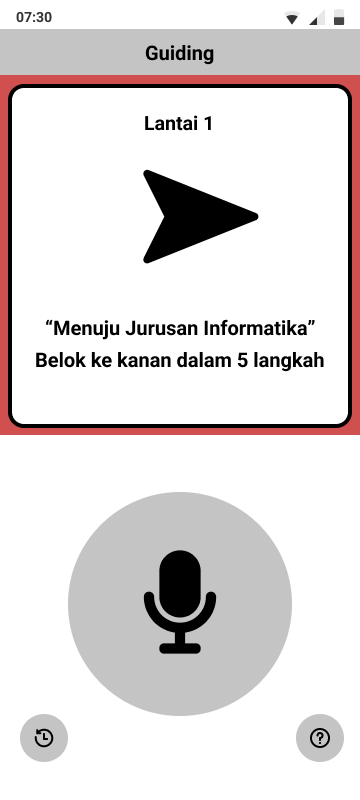
\includegraphics[width=.5\linewidth]{gambar/bab3/3}  
  		\caption{Proses Navigasi ke Tujuan}
	\end{subfigure}
	\begin{subfigure}{.5\textwidth}
  		\centering
  		% include fourth image
  		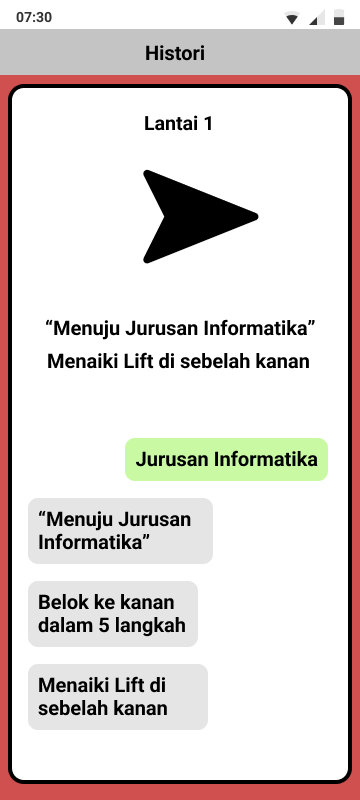
\includegraphics[width=.5\linewidth]{gambar/bab3/4}  
  		\caption{Histori Navigasi}
	\end{subfigure}
		\vspace{0.5cm}
		\caption{Tampilan Halaman Aplikasi Navigasi Indoor untuk Tunanetra}
	\label{aplikasimappingbagian1}
	\end{figure}

\end{enumerate}

%%%%%%%%%%%%%%%%%%%%%%%%%%%%%%%%%%%%%%%%%

\subsection{Pengumpulan Data}
\begin{enumerate}
\item Data Model \textit{Voice Recognition}
\par Data yang digunakan dalam penelitian ini terdiri atas data \textit{pre-trained} model yang diperoleh dari penelitian yang berada dalam satu penelitian yang sama pada \textit{roadmap} pada gambar \ref{img:fase2}. \textit{Pre-trained} model dimanfaatkan sebagai titik awal untuk merespons perintah suara dari pengguna, kemudian perintah suara akan di terjemahkan ke dalam bentuk teks yang akan diterima oleh \textit{smartphone} pengguna. Teks yang diterima akan digunakan sebagai input yang akan menjadi lokasi tujuan serta pemilihan rute.

\item Data Rute dan Denah Lokasi Penelitian
\par Rute yang akan digunakan berlokasi di gedung A FMIPA lantai 1 sampai dengan lantai 3. Data rute yang digunakan akan di petakan dengan menggunakan bantuan BLE. Data titik-titik BLE disimpan dalam \textit{database} lokal berupa MAC \textit{Address}, nilai RSSI, dan nama perangkat BLE. Dengan adanya RSSI atau kekuatan sinyal yang disimpan perangkat smartphone pengguna akan menangkap sinyal dan menyesuaikan dengan titik-titik yang telah dipetakan sehingga mendapatkan lokasi pengguna berada serta menjadikan titik lokasi pengguna sebagai pemilihan rute terdekat ke lokasi tujuan pengguna. Denah lokasi penelitian dapat dilihat pada gambar berikut.

\begin{figure}[H]
\centering
{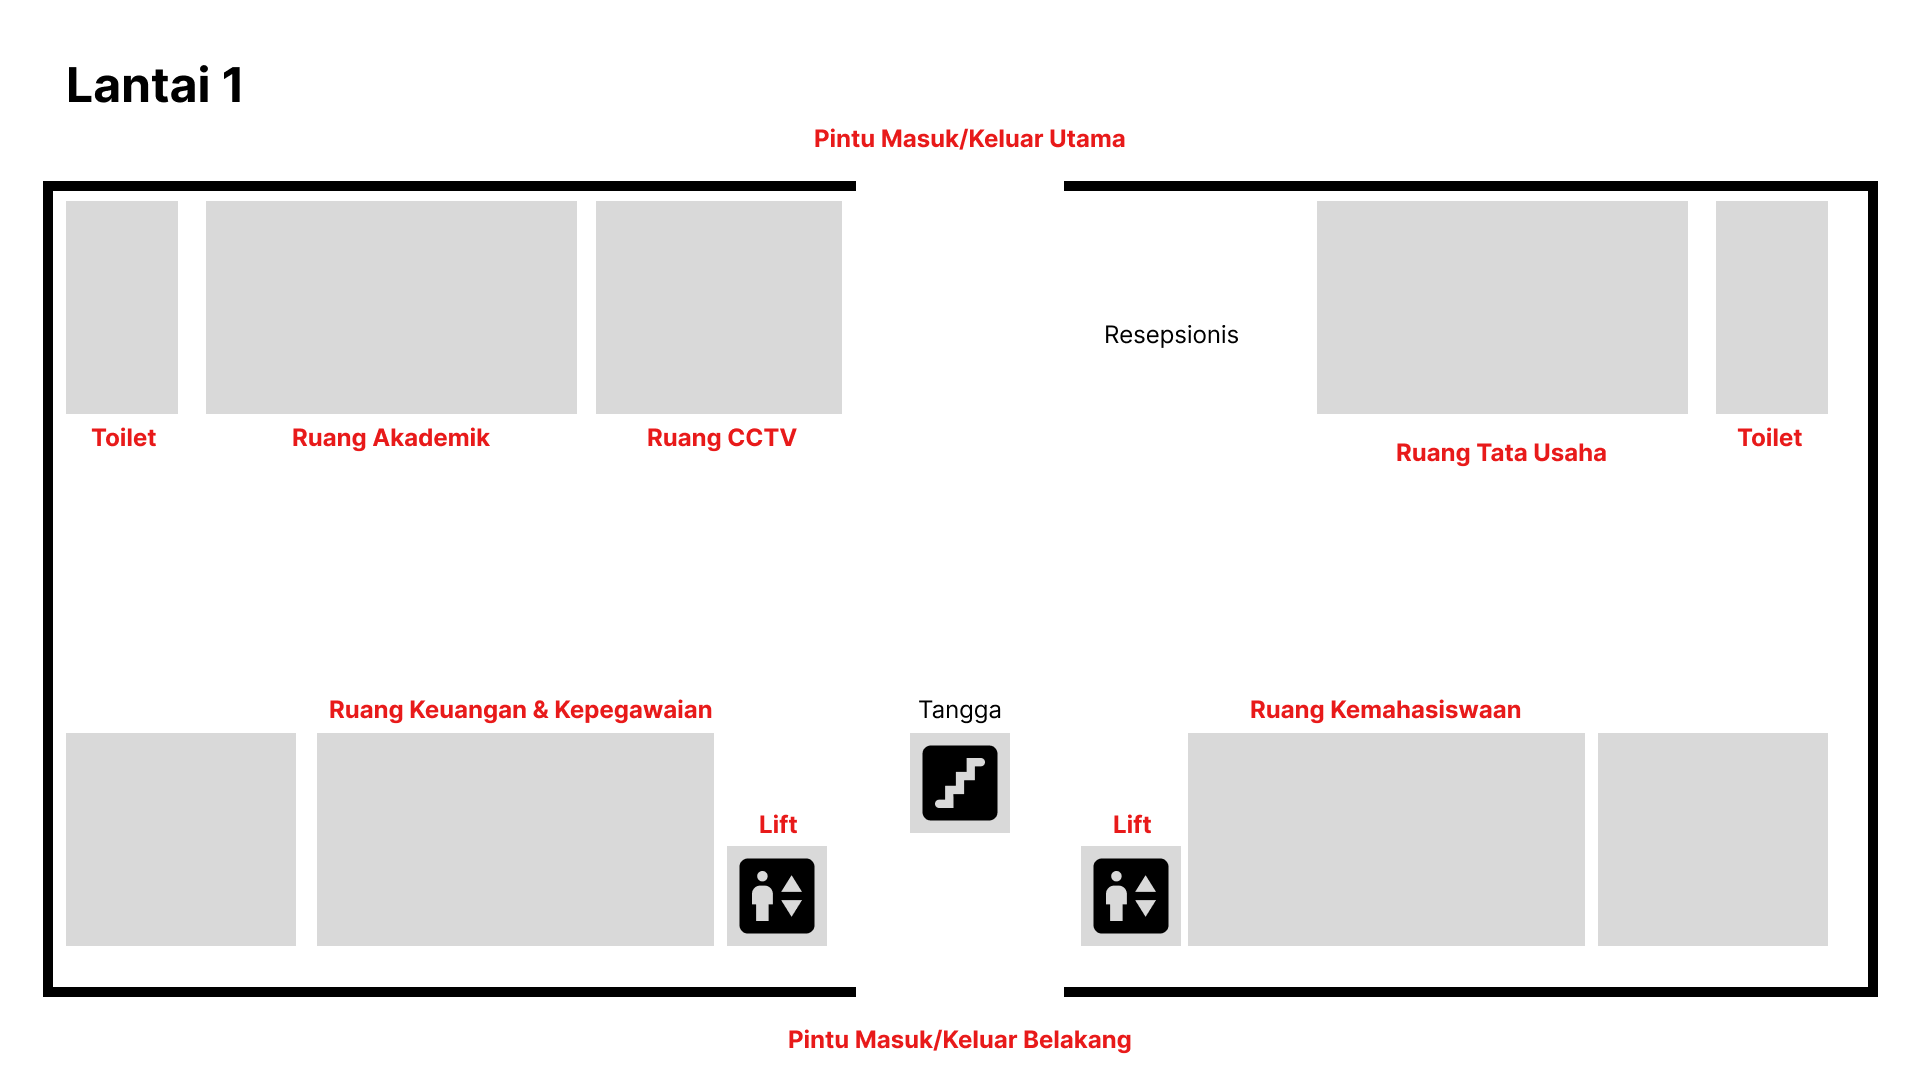
\includegraphics [scale = 0.2]{gambar/bab3/Denah-1}}
\caption{Denah lantai 1 Gedung A FMIPA}
\label{img:denah_1}
\end{figure}

\begin{figure}[H]
\centering
{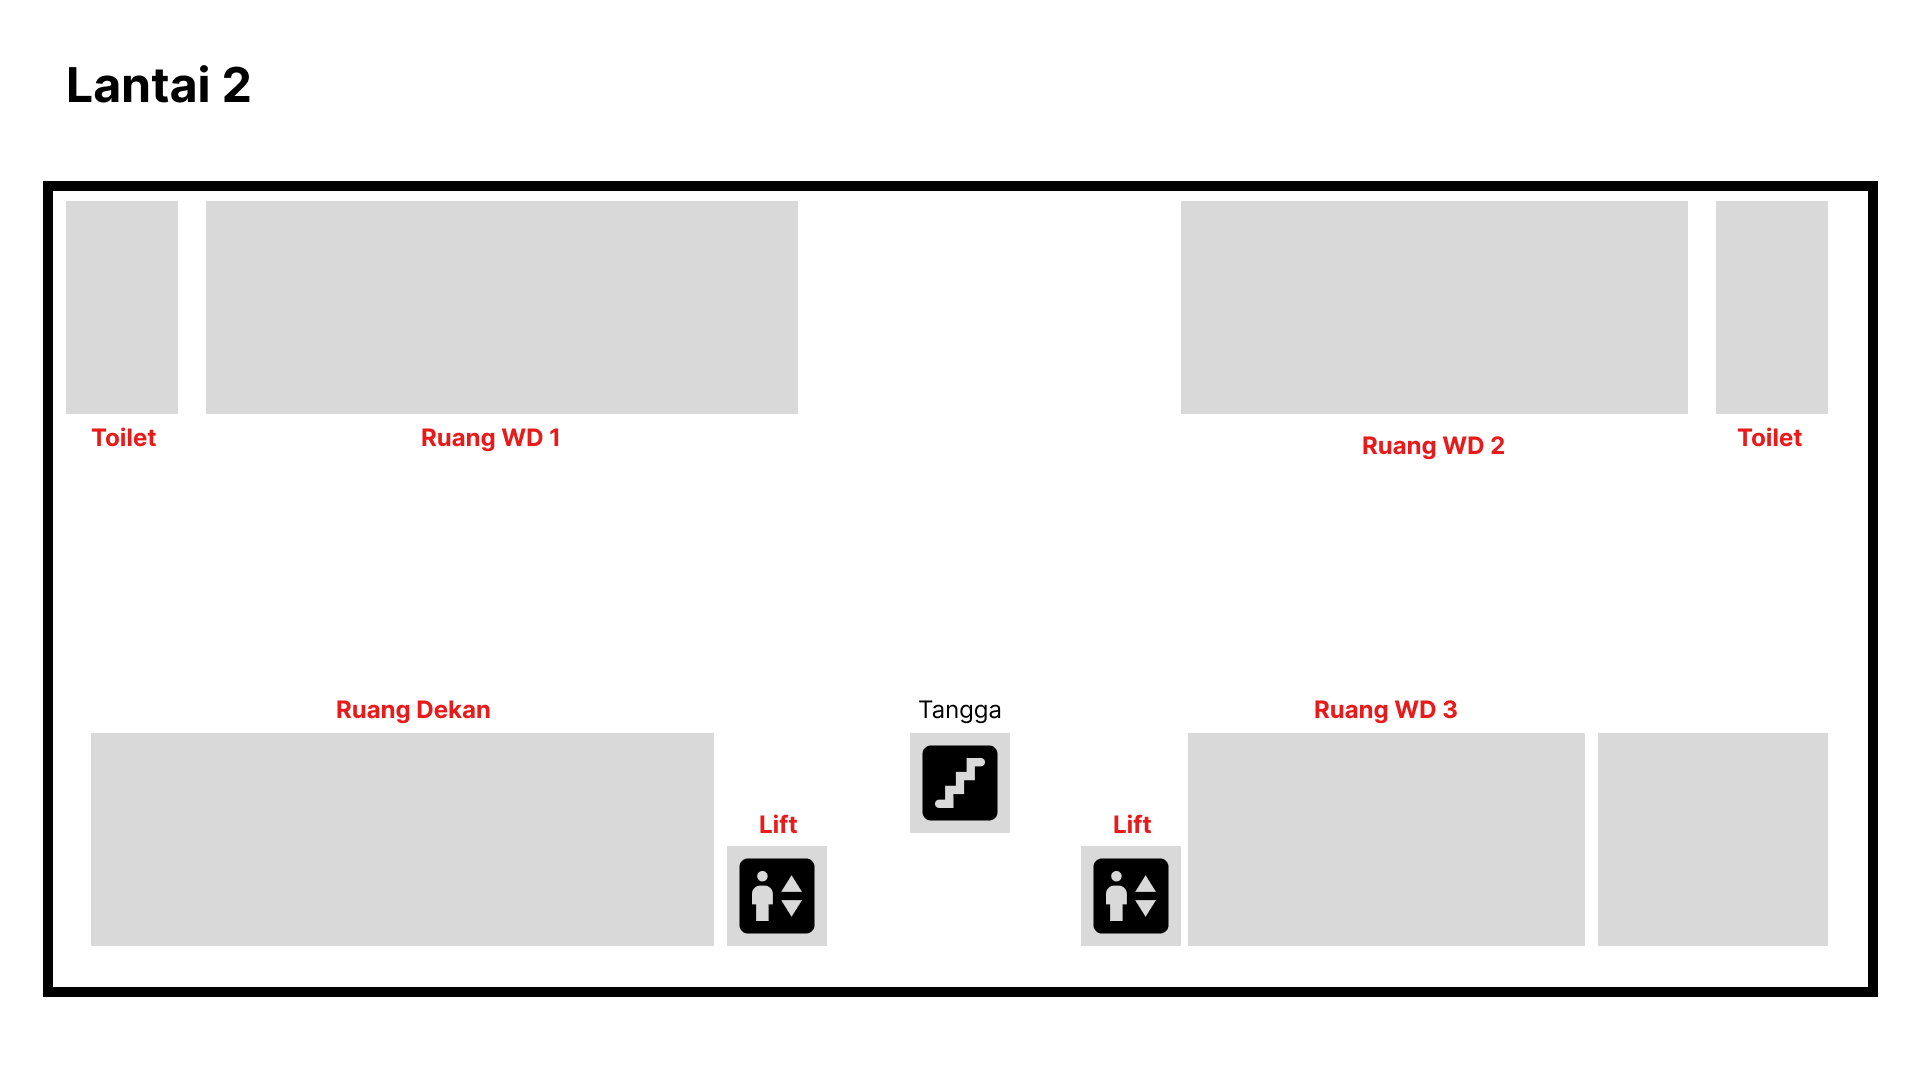
\includegraphics [scale = 0.2]{gambar/bab3/Denah-2}}
\caption{Denah lantai 2 Gedung A FMIPA}
\label{img:denah_2}
\end{figure}

\begin{figure}[H]
\centering
{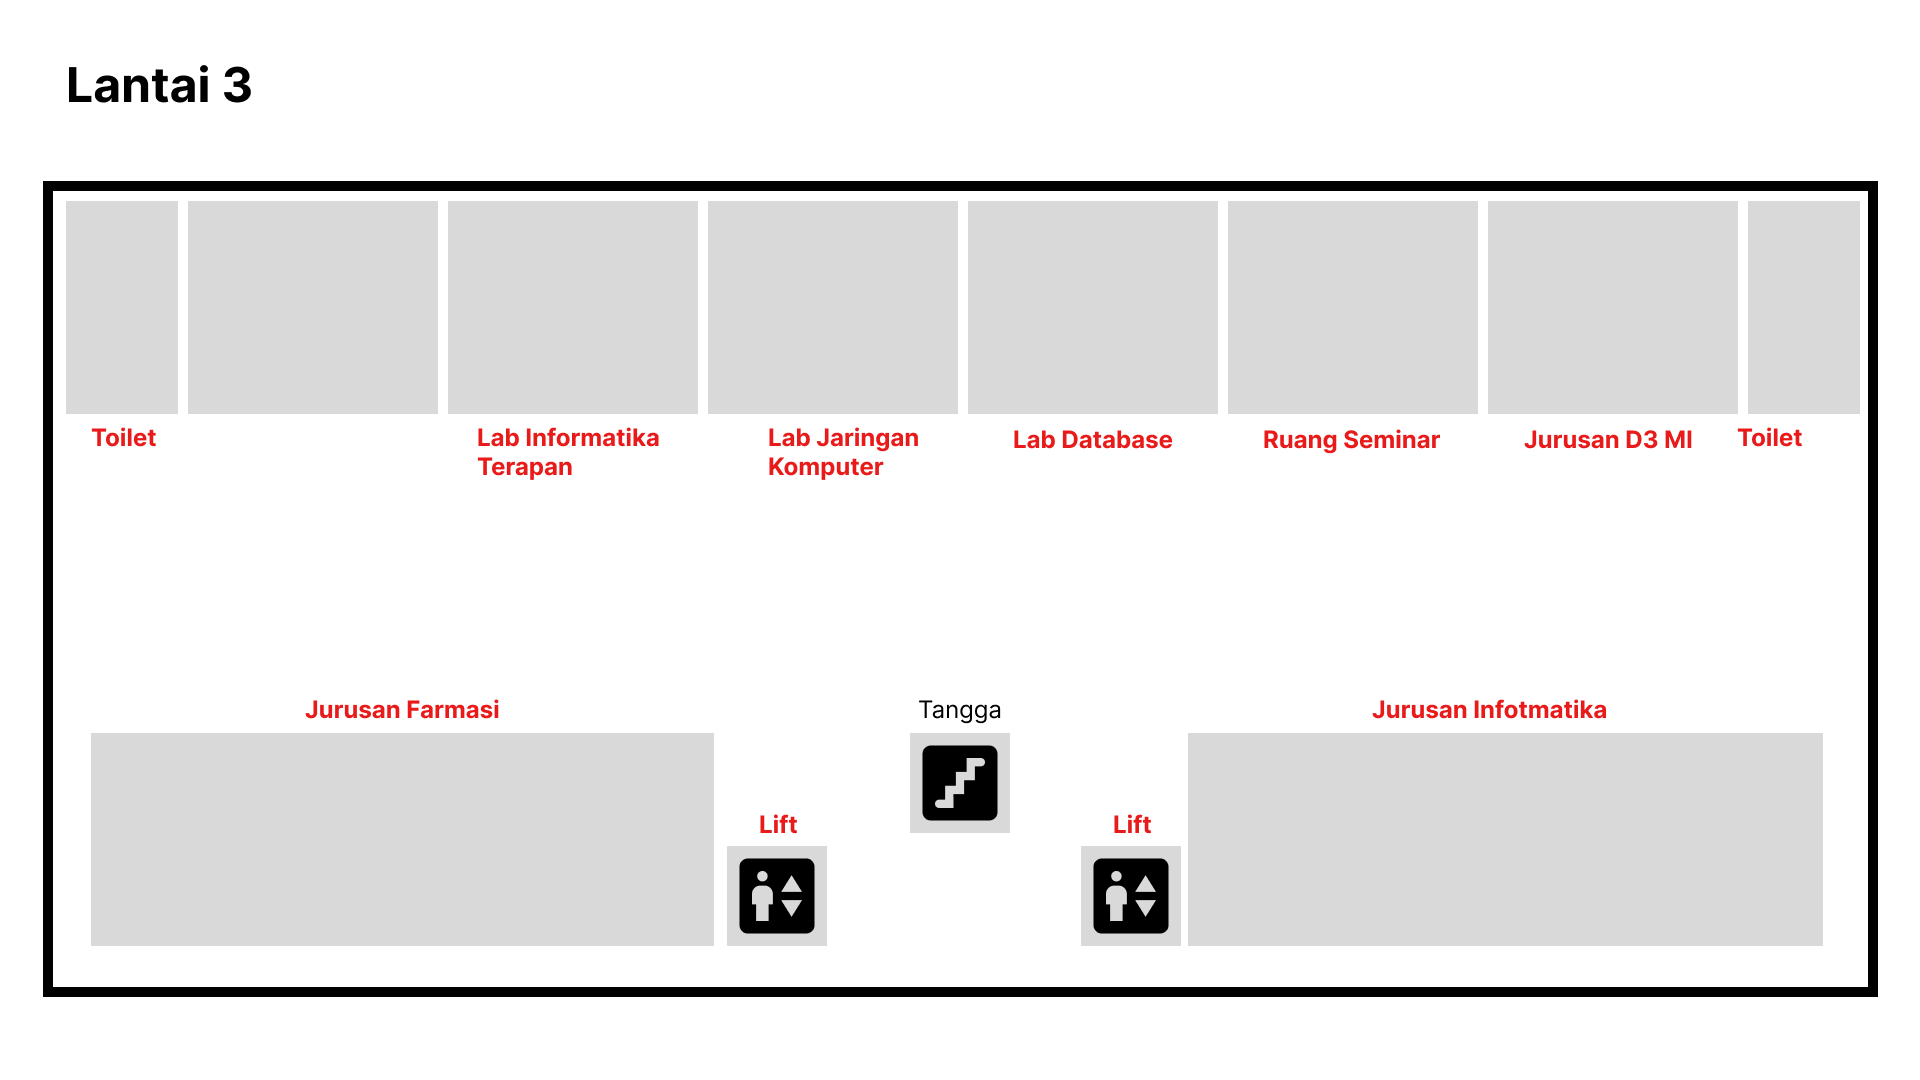
\includegraphics [scale = 0.2]{gambar/bab3/Denah-3}}
\caption{Denah lantai 3 Gedung A FMIPA}
\label{img:denah_3}
\end{figure}


\item Data \textit{Text-to-Speech}
\par Data yang akan digunakan menggunakan \textit{text-to-speech} yang disediakan oleh library Google speech. Sehingga proses pemanduan menuju ruangan akan dipandu dengan suara seperti "Menuju Ruangan Jurusan Informatika", "Belok ke kanan dalam 5 langkah", "Telah sampai di tujuan , Ruangan Jurusan Informatika".

\newpage
\item Data akurasi lokasi pengguna serta akurasi rute
\par Data yang akan diperoleh dari proses koneksi BLE terdekat dengan RSSI sebagai tolak ukur akurasi lokasi pengguna, sedangkan untuk akurasi rute menggunakan data pemetaan rute dan lokasi tujuan yang telah dipetakan pada aplikasi dengan memanfaatkan RSSI dari beberapa koneksi BLE terdekat yang saling terhubung menggunakan Kalman Filter.

\end{enumerate}


\subsection{Pembuatan Sistem Aplikasi}
Pada Proses pembuatan sistem aplikasi, metode pengembangan aplikasi yang digunakan adalah metode \textit{Scrum}, dikarenakan sistem ini dikembangkan bersama dengan tim dan membutuhkan fleksibilitas terhadap perubahan yang terjadi dalam proses pengembangannya, sehingga memerlukan iterasi secara berkala agar berjalan dengan baik. Salah satu tahap yang merupakan paling awal dari metode ini adalah \textit{product backlog}. Pada tahap ini, semua kebutuhan akan ditransformasikan menjadi rancangan pekerjaan untuk diselesaikan agar aplikasi dapat bekerja secara fungsional. Adapun \textit{product backlog} dari keseluruhan aplikasi ini adalah sebagai berikut.

\begin{itemize}
\item Menampilkan halaman beranda.

\item Menampilkan \textit{Pop up} yang muncul dari \textit{input} suara.

\item Meluncurkan aplikasi dengan proses pengenalan suara.

\item Menampilkan dan mengeluarkan suara daftar ruangan yang bisa di gunakan sebagai tujuan.

\item Menampilkan rute terdekat ke ruangan yang di tuju oleh pengguna.

\item Mengeluarkan suara navigasi ke ruangan yang di tuju.

\end{itemize}

\subsection{Pengujian Akurasi}
Pengujian akurasi posisi pengguna dan pemilihan rute akan menggunakan gabungan titik BLE sebagai titik awal dengan mengukur kekuatan RSSI, kemudian menggunakan letak dan posisi BLE yang telah dipetakan sebelumnya untuk melakukan pemilihan rute serta proses navigasi yang akan diprediksi menggunakan algoritma Kalman Filter disertai dengan fase pembaharuan prediksi titik lokasi pengguna ke tujuan.

\newpage
Berikut perhitungan yang akan digunakan untuk menguji akurasi pengguna serta rute pengguna, rumus menurut \citep{ihsan2018analisis}:
\begin{itemize}
\item \textit{Time Update (Predict)}

\par \textit{Predict State}
\begin{equation}
x = x
\end{equation}

\par \textit{Predict error covariance}
\begin{equation}
p = p + q
\end{equation}

\item \textit{Measurements update (Correct)}
\par \textit{Update the estimate via} k 
\begin{equation}
x = x + k*(measurement – x)
\end{equation}

\par Kalman \textit{gain} 
\begin{equation}
k = p / ( p+r )
\end{equation}

\par \textit{Update the error covariance}
\begin{equation}
p = (1 – k )* p
\end{equation}

\end{itemize}
\par Keterangan
\par x: Nilai yang di filter
\par p: Error estimasi
\par q: Noise yang diakibatkan dari proses
\par k: Kalman Gain
\par r: Noise dari sensor\newline

\subsection{Pengujian Fungsionalitas dengan Metode \textit{Black Box}}
Metode yang digunakan untuk melakukan pengujian fungsionalitas adalah dengan \textit{black box testing}. Pengujian ini dilakukan untuk memeriksa fungsi-fungsi pada sistem yang dibangun pada penelitian ini apakah sudah bekerja sesuai dengan kebutuhan pengguna ataupun tidak. Pengujian ini dilakukan dengan cara menjalankan setiap fungsi yang ada pada sistem dan memastikan agar sistem dapat bekerja dengan semestinya sesuai alur yang telah dirancang. Pengujian ini juga dapat melibatkan target pengguna dan pengembang.

\subsection{\textit{Usability Testing}}
\textit{Usability Testing} merupakan pengujian aplikasi untuk melihat apakah pengguna dapat dengan mudah dan nyaman dalam menggunakan aplikasi tersebut serta melihat dan mengevaluasi keberhasilan dari sebuah produk atau jasa. Pengujian ini akan menggunakan metode UMUX. UMUX terdiri dari 4 pertanyaan dengan menggunakan skala 1-7. Berikut daftar pertanyaan-pertanyaan dengan metode UMUX dapat dilihat pada Tabel \ref{tab:UMUX}.

\begin{table}[H]
\caption{Daftar Pertanyaan Metode UMUX.}
\label{tab:UMUX}
\resizebox{\columnwidth}{!}{%
\begin{tabular}{|l|l|}
\hline
1 & Kemampuan sistem ini memenuhi persyaratan saya.                  \\ \hline
2 & Menggunakan sistem ini adalah
pengalaman yang membuat frustrasi.  \\ \hline
3 & Sistem ini mudah digunakan.                                       \\ \hline
4 & Saya harus menghabiskan terlalu banyak waktu untuk
memperbaiki hal-hal dengan sistem ini. \\ \hline
\end{tabular}%
}
\end{table}

Untuk menghitung skor akhir metode UMUX \citep{finstad2010usability}, dapat dilihat dari cara berikut.

\begin{enumerate}
\item Item ganjil diberi skor [ skor pengguna - 1]. Item genap diberi skor [7 - skor pengguna].

\item Jumlahkan perbedaan ini dan bagi jumlahnya dengan 24 (skor tertinggi).

\item Kalikan hasil dengan 100.

\item Cari nilai rata-rata dari seluruh pengguna.
\end{enumerate}

\par Tingkat nilai skala pengujian menentukan apakah sistem tersebut layak digunakan, bermanfaat, diterima oleh pengguna dan bertahan lama penggunaannya. Sebuah sistem dengan nilai pengujian yang tinggi membuat sistem tersebut menjadi populer dalam waktu yang lama dan penggunaannya yang luas, dikarenakan banyak individu akan merasakan manfaat dari kehadiran sistem tersebut. Sedangkan sistem dengan nilai pengujian yang rendah, sering kali diabaikan walaupun dibuat berdasarkan kebutuhan dan menghasilkan sumber daya yang banyak.



%-----------------------------------------------------------------------------%

% Baris ini digunakan untuk membantu dalam melakukan sitasi
% Karena diapit dengan comment, maka baris ini akan diabaikan
% oleh compiler LaTeX.
\begin{comment}
\bibliography{daftar-pustaka}
\end{comment}

%-------------------------------------------------------------------------------
%                            BAB IV
%               		HASIL DAN PEMBAHASAN
%-------------------------------------------------------------------------------
\fancyhf{} 
\fancyfoot[C]{\thepage}
\chapter{HASIL DAN PEMBAHASAN}

\section{Persiapan Sistem}
\subsection{Dataset}
	\begin{enumerate}
	\item Data Model \textit{Voice Recognition}
	\par Data yang digunakan dalam penelitian ini terdiri atas data \textit{pre-trained} model yang diperoleh dari penelitian yang berada dalam satu penelitian yang sama pada \textit{roadmap} pada gambar \ref{img:fase2}. \textit{Pre-trained} model dimanfaatkan sebagai titik awal untuk merespons perintah suara dari pengguna, kemudian perintah suara akan di terjemahkan ke dalam bentuk teks yang akan diterima oleh \textit{smartphone} pengguna. Teks yang diterima akan digunakan sebagai input yang akan menjadi lokasi tujuan serta pemilihan rute. Berikut adalah \textit{list} dari nama-nama ruangan yang ada pada data \textit{Pre-trained} model.
	
	
	\begin{longtable}{| m{1cm} | m{6cm} | m{3cm} |}
    \caption{Data Ruangan}
    \label{t_data} \\
        \hline
        \textbf{No.}	& \textbf{Nama Ruangan}	& \textbf{keterangan}	\\
        \hline
		1.	& ruang cctv & \multirow{6}{*}{Lantai 1} \\ \cline{1-2}
		2.  & ruang kepegawaian					& \\ \cline{1-2}
		3.	& ruang tata usaha					& \\ \cline{1-2}
		4.	& ruang tu							& \\ \cline{1-2}
		5.	& ruang kemahasiswaan				& \\ \cline{1-2}
		6.	& ruang akademik					& \\
        \hline
        7.	& ruang dekan & \multirow{7}{*}{Lantai 2} \\ \cline{1-2}
		8.  & ruang wakil dekan satu			& \\ \cline{1-2}
		9.	& ruang wd satu						& \\ \cline{1-2}
		10.	& ruang wakil dekan dua				& \\ \cline{1-2}
		11.	& ruang wd dua						& \\ \cline{1-2}
		12.	& ruang wakil dekan tiga			& \\ \cline{1-2}
		13.	& ruang wd tiga						& \\ 
		\hline
		14.	& jurusan informatika & \multirow{7}{*}{Lantai 3} \\ \cline{1-2}
		15.	& jurusan d tiga mi					& \\ \cline{1-2}
		16. & jurusan farmasi					& \\ \cline{1-2}
		17.	& ruang seminar						& \\ \cline{1-2}
		18.	& laboratorium jaringan komputer	& \\ \cline{1-2}
		19.	& lab jaringan komputer				& \\ \cline{1-2}
		20.	& laboratorium jaringan				& \\ \cline{1-2}
		21. & lab jaringan						& \\ \cline{1-2}
		22.	& laboratorium jarkom				& \\ \cline{1-2}
		23.	& lab jarkom						& \\ \cline{1-2}
		24.	& laboratorium basis data			& \\ \cline{1-2}
		25.	& lab basis data					& \\ \cline{1-2}
		26.	& laboratorium data mining			& \\ \cline{1-2}
		27.	& lab data mining					& \\ \cline{1-2}
		28. & laboratorium multimedia			& \\ \cline{1-2}
		29.	& lab multimedia					& \\ \cline{1-2}
		30.	& laboratorium gis					& \\ \cline{1-2}
		31.	& lab gis							& \\ 
		\hline
		32.	& ruang wakil dekan tiga & \multirow{24}{*}{Ruangan Umum} \\ \cline{1-2}
		33.  & ruang wakil dekan satu			& \\ \cline{1-2}
		34.	& ruang wd satu						& \\ \cline{1-2}
		35.	& ruang wakil dekan dua				& \\ \cline{1-2}
		36.	& ruang wd dua						& \\ \cline{1-2}
		37.	& ruang wakil dekan tiga			& \\ \cline{1-2}
		38.	& ruang seminar						& \\ \cline{1-2}
		39.	& laboratorium jaringan komputer	& \\ \cline{1-2}
		40.	& lab jaringan komputer				& \\ \cline{1-2}
		41. & lab jaringan						& \\ \cline{1-2}
		42.	& laboratorium jarkom				& \\ \cline{1-2}
		43.	& lab jarkom						& \\ \cline{1-2}
		44.	& laboratorium basis data			& \\ \cline{1-2}
		45.	& lab basis data					& \\ \cline{1-2}
		46.	& laboratorium data mining			& \\ \cline{1-2}
		47.	& lab data mining					& \\ \cline{1-2}
		48. & laboratorium multimedia			& \\ \cline{1-2}
		49.	& lab multimedia					& \\ \cline{1-2}
		50.	& laboratorium gis					& \\ \cline{1-2}
		51. & lab jaringan						& \\ \cline{1-2}
		52.	& laboratorium jarkom				& \\ \cline{1-2}
		53.	& lab jarkom						& \\ \cline{1-2}
		54.	& laboratorium basis data			& \\ \cline{1-2}
		55.	& lab basis data					& \\ \cline{1-2}
		56.	& laboratorium data mining			& \\ 
        \hline
    \end{longtable}
	
	\newpage
	
	\item Data Rute dan Denah Lokasi Penelitian
	\par Rute yang akan digunakan berlokasi di gedung A FMIPA lantai 1 sampai dengan lantai 3. Data rute yang digunakan akan dipetakan dengan menggunakan bantuan BLE. Data titik-titik BLE disimpan dalam \textit{database} lokal berupa MAC \textit{Address}, nilai RSSI, dan nama perangkat BLE. BLE berjumlah 40 unit dengan BLE untuk ruangan berjumlah 24 ditandai dengan titik berwarna hijau dan BLE untuk \textit{connector} berjumlah 16 ditandai dengan titik berwarna biru.Jarak masing-masing BLE berada di sekitar 5 s/d 8 meter dari masing-masing BLE. Denah lokasi penelitian dapat dilihat pada gambar berikut.
	
	\begin{figure}[H]
\centering
{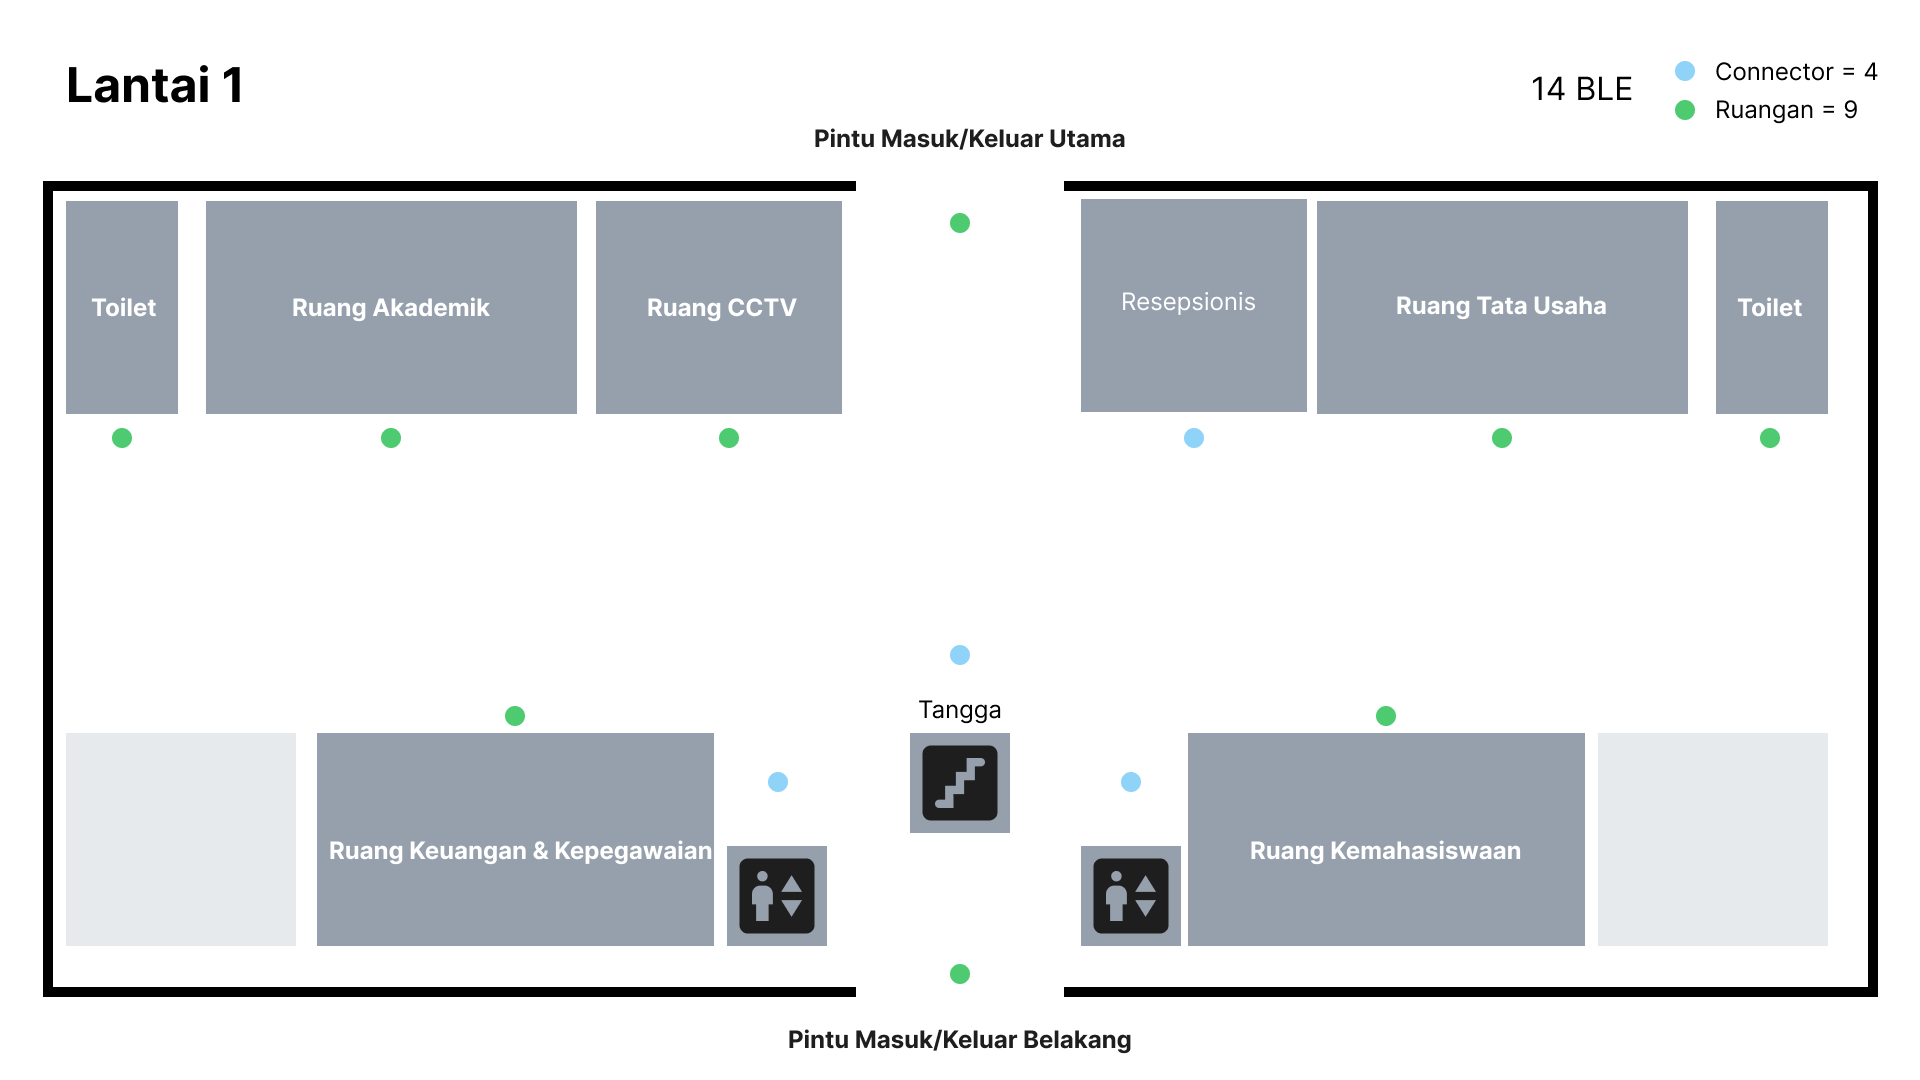
\includegraphics [scale = 0.2]{gambar/bab4/Denah-1-BLE}}
\caption{Denah lantai 1 Gedung A FMIPA dengan BLE}
\label{img:denah_1_ble}
\end{figure}

\begin{figure}[H]
\centering
{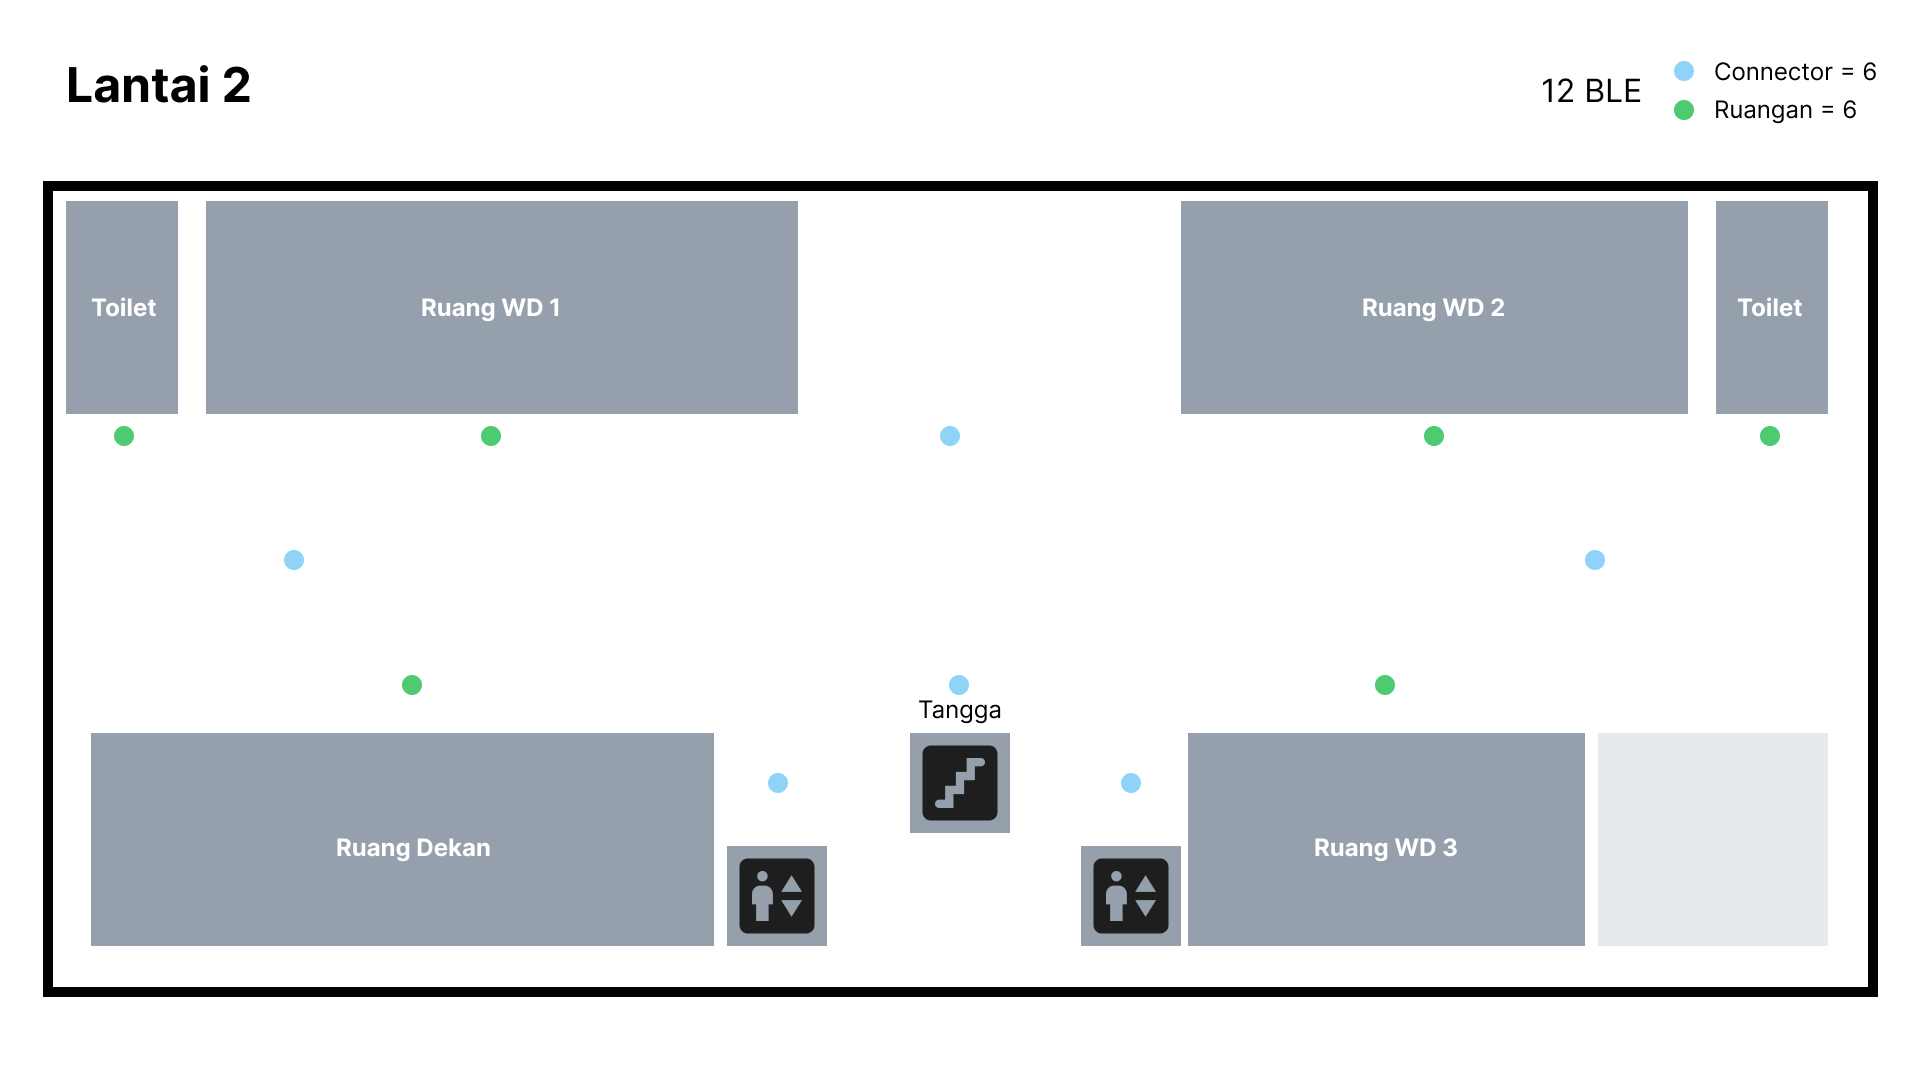
\includegraphics [scale = 0.2]{gambar/bab4/Denah-2-BLE}}
\caption{Denah lantai 2 Gedung A FMIPA dengan BLE}
\label{img:denah_2_ble}
\end{figure}

\begin{figure}[H]
\centering
{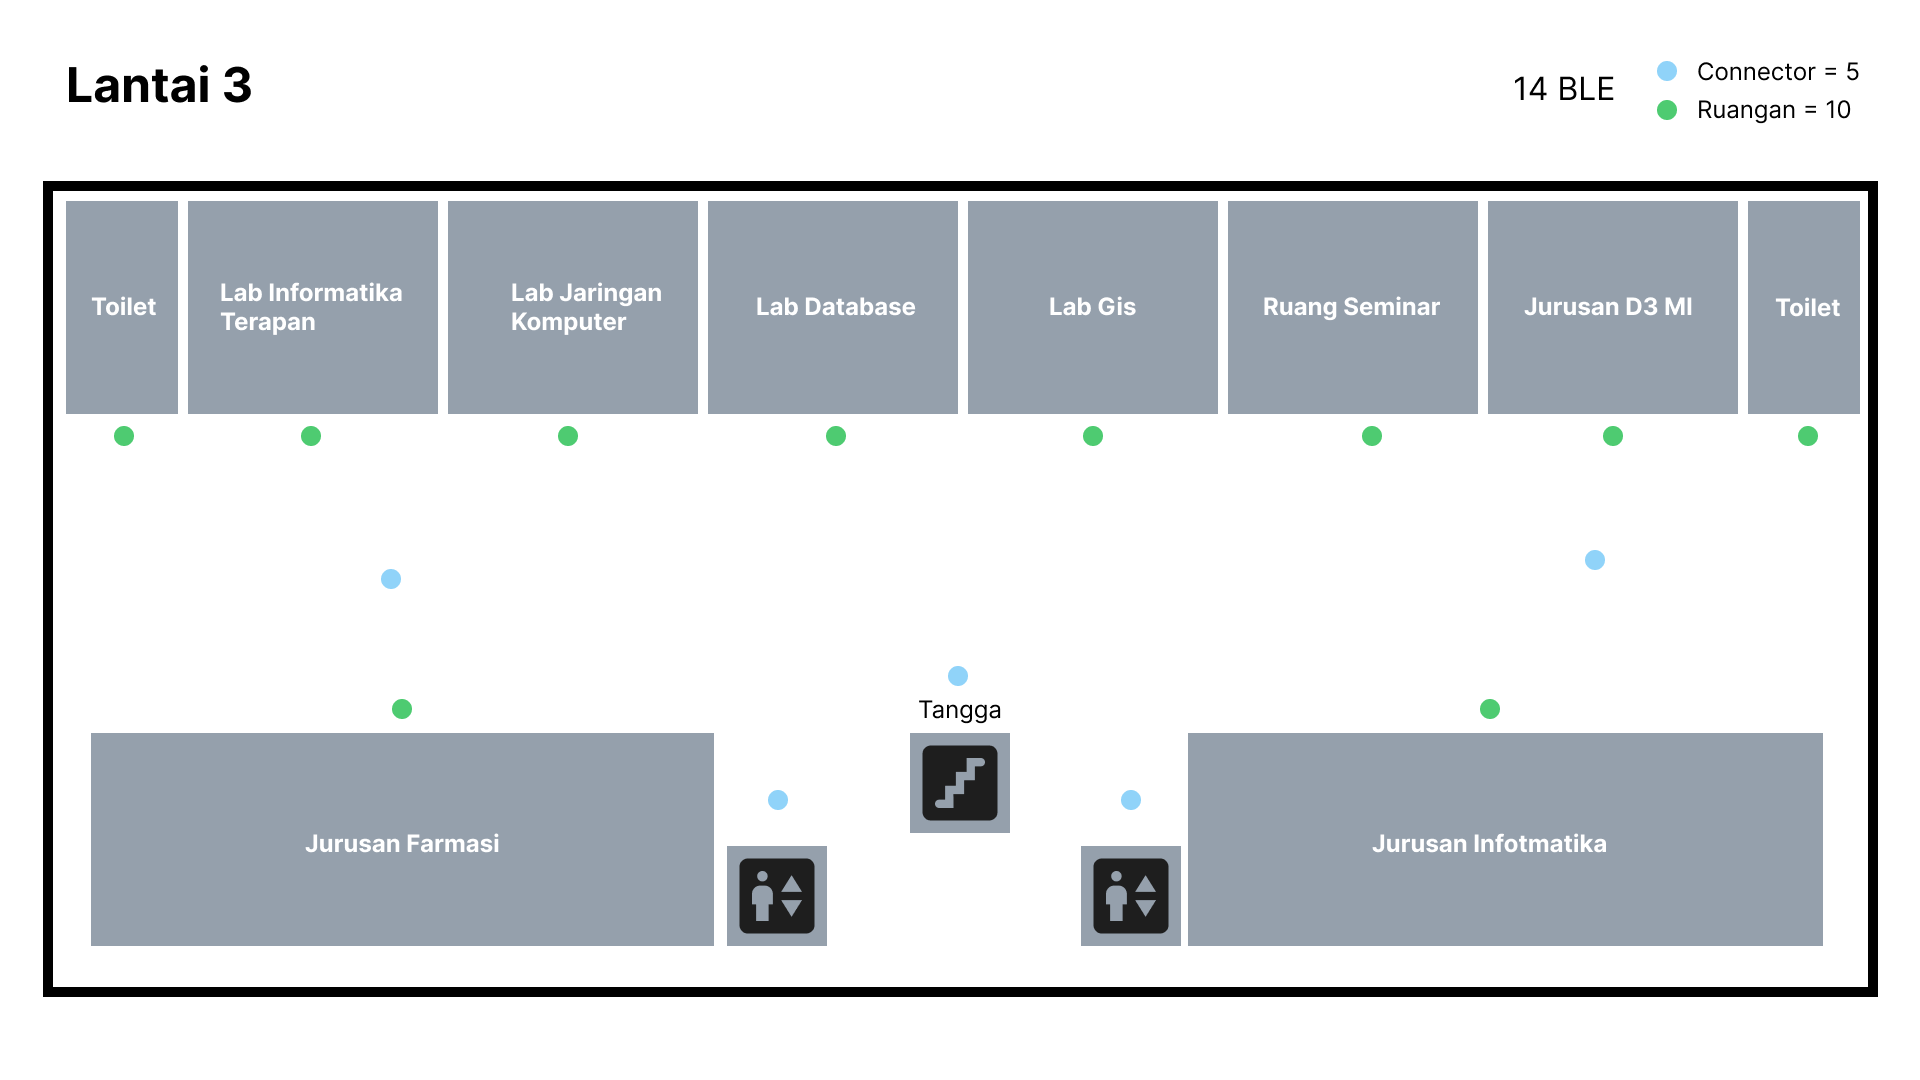
\includegraphics [scale = 0.2]{gambar/bab4/Denah-3-BLE}}
\caption{Denah lantai 3 Gedung A FMIPA dengan BLE}
\label{img:denah_3_ble}
\end{figure}
    
	\end{enumerate}
	
	
	
	
\subsection{Pembangunan Sistem}
	\begin{enumerate}
	
	\item Konfigurasi Model \textit{Voice Recognition} dan \textit{Text-to-speech}
	\par Pada tahapan ini model dipasangkan ke dalam aplikasi dengan menggunakan VOSK API dan Google \textit{text-to-speech} dengan menggunakan fungsi Talkback pada Android sehingga aplikasi dapat menerima input dari pengguna serta memberikan informasi \textit{feedback} ke pengguna saat dipandu.
	
	\newpage
	\item  Data akurasi lokasi pengguna serta akurasi rute
\par Data yang akan diperoleh dari proses koneksi BLE terdekat dengan RSSI sebagai tolak ukur akurasi lokasi pengguna, sedangkan untuk akurasi rute menggunakan data pemetaan rute dan lokasi tujuan yang telah dipetakan pada aplikasi dengan memanfaatkan RSSI dari beberapa koneksi BLE terdekat yang saling terhubung menggunakan Kalman Filter.

	\item Pembuatan Aplikasi
	\par Aplikasi dibuat dengan menggunakan bahasa pemrograman Kotlin dengan menggunakan \textit{jetpack compose} melalui IDE Android Studio. Media penyimpanan data BLE dan lokasi menggunakan basis data ROOM. Basis data disimpan secara lokal dan dapat diakses menggunakan query MySQL berbasis DAO ROOM. BLE dan data lokasi tersimpan berupa Id, RSSI, MAC Address, nama ruangan. Proses input pengguna dapat memanggil aplikasi secara langsung menggunakan suara dan memberi lokasi tujuan. Titik mulai pengguna diakses menggunakan Bluetooth dengan mencari BLE terdekat dengan lokasi pengguna.
	
	\vspace{-0cm}
	\begin{figure} [H]
	\begin{subfigure}{.5\textwidth}
 		\centering
 		% include first image
 		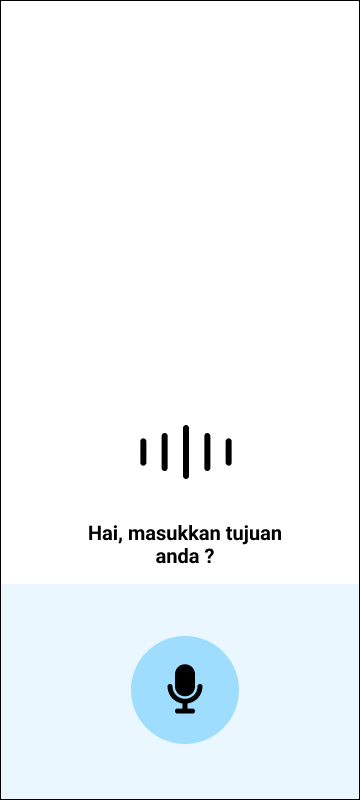
\includegraphics[width=.5\linewidth]{gambar/bab4/pandu-pop-up} 
 		\caption{Pop up trigger by hotword}
	\end{subfigure}
	\begin{subfigure}{.5\textwidth}
 		\centering
 		% include second image
		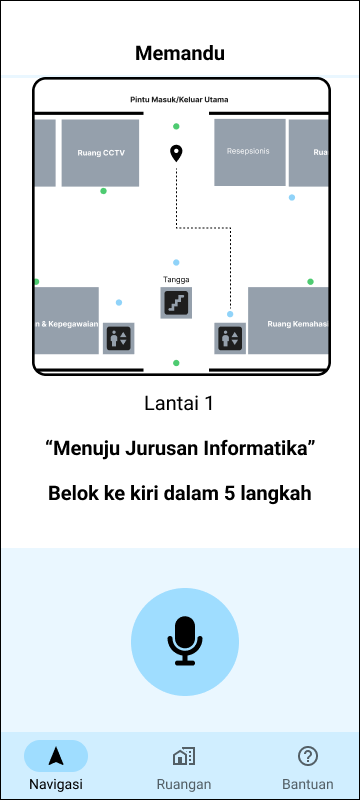
\includegraphics[width=.5\linewidth]{gambar/bab4/memandu} 
 		\caption{Input tujuan dan lokasi pengguna}
	\end{subfigure}
		\vspace{1cm}
		\newline
	\begin{subfigure}{.5\textwidth}
 		\centering
		 % include third image
	  	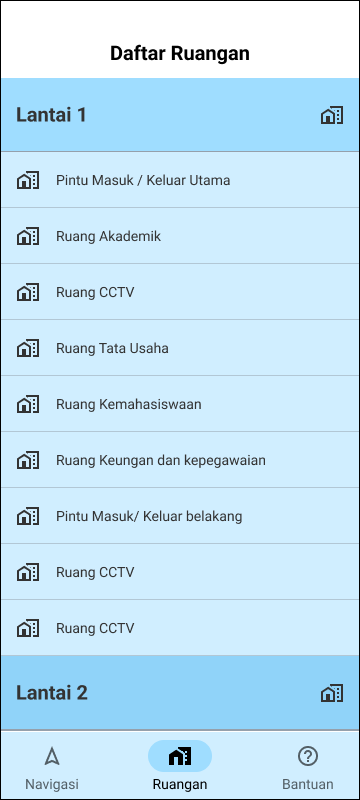
\includegraphics[width=.5\linewidth]{gambar/bab4/daftar-ruangan} 
 		\caption{Daftar Ruangan}
	\end{subfigure}
	\begin{subfigure}{.5\textwidth}
 		\centering
 		% include fourth image
 		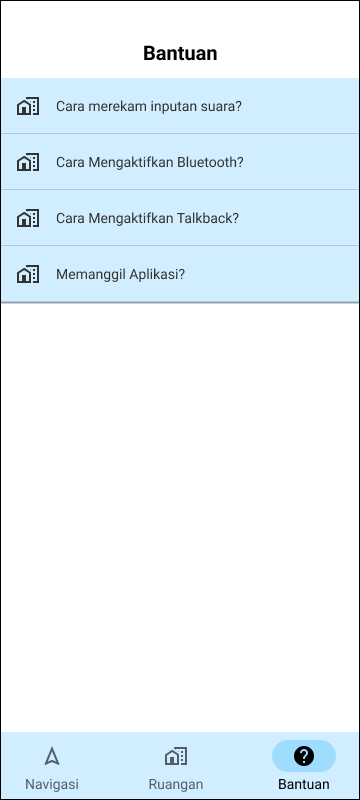
\includegraphics[width=.5\linewidth]{gambar/bab4/bantuan} 
 		\caption{Bantuan}
	\end{subfigure}
		\vspace{0.5cm}
		\caption{Tampilan Halaman Aplikasi Navigasi Indoor untuk Tunanetra}
	\label{aplikasimappingbagian1}
	\end{figure}

\end{enumerate}

\newpage
\section{Pengujian Sistem}
\subsection{Akurasi rute}
\par Pengujian akurasi posisi dan rute pengguna menggunakan gabungan titik BLE terdekat dengan mengukur kekuatan RSSI, kemudian menggunakan letak dan posisi BLE yang telah dipetakan dengan menghitung menggunakan Kalman Filter yang disertai dengan pembaharuan prediksi titik lokasi pengguna ke tujuan dan menghingtung kesalahan prediksi dan estimasi dengan data aktual.
Pengujian menggunakan 3 skema pengujian yang di uji pada 5 pengguna tunanetra seperti pada Tabel \ref{tab:skema-pengujian} berikut




\begin{table}[H]
\caption{Skema Pengujian Akurasi Pengambilan Rute di Gedung A FMIPA Optimal dalam MSE \textit{(Mean Squared Error)}}
\label{tab:skema-pengujian}
\resizebox{\columnwidth}{!}{
\begin{tabular}{|c|c|c|c|c|c|c|c|c|}
\hline
\textbf{No.} & \textbf{Titik Awal} & \textbf{Tujuan} & \textbf{Pengguna 1} & \textbf{Pengguna 2} & \textbf{Pengguna 3} & \textbf{Pengguna 4} & \textbf{Pengguna 5} & \textbf{Rute Optimal} \\ \hline
1 & Pintu masuk utama   & Toilet lantai 1     & 1.252 & 10.254 & 3.325 & 2.902 & 0.873 & 0.577 \\ \hline
2 & Pintu masuk utama   & Jurusan Informatika & 4.213 & 6.321  & 3.126 & 4.234 & 5.432 & 2.332 \\ \hline
3 & Jurusan Informatika & Pintu Keluar Utama  & 5.432 & 4.213  & 6.783 & 5.126 & 4.786 & 2.213 \\ \hline
\end{tabular}
}
\end{table}

\par Data Aktual berupa data pengembang dengan menggunakan perhitungan jarak BLE berdasarkan jarak antar BLE dan tujuan akhir secara langsung secara berurut mengikuti BLE terdekat, didapati MSE \textit{(Mean Squared Error)} seperti pada Tabel \ref{tab:skema-pengujian}. Terdapat pengguna mendapati rute yang mendekati rute optimal yang dipilih oleh aplikasi, sehingga pengguna yang mendekati rute optimal memiliki MSE rendah yang berarti mendekati akurat. Terdapat juga pengguna yang memiliki MSE tinggi dapat dipengaruhi oleh beberapa faktor seperti sinyal BLE, lokasi BLE, tembok, lokasi pengguna, dan saran rute yang diberikan melewati rute yang jauh dari rute optimal.

\newpage
\subsection{Pengujian Usabilitas UMUX}
\par Pengujian usabilitas bertujuan untuk menguji kelayakan dan kegunaan dari sistem yang akan digunakan oleh pengguna. Sebelum pengujian ini dilakukan, adapun skema pengujian yang telah dibuat dapat dilihat pada Tabel \ref{tab:skema-pengujian}.

\par Pengujian dengan metode UMUX dilakukan dengan menanyakan pertanyaan kepada responden. Kuesioner berisi 4 pertanyaan dengan menggunakan skala 1-7. Hasil pengujian UMUX aplikasi dapat dilihat pada Tabel \ref{tab:skor-umux} berikut.

% Please add the following required packages to your document preamble:
% \usepackage{multirow}
\begin{table}[H]
\caption{Hasil Pengujian UMUX Aplikasi Navigasi}
\label{tab:skor-umux}
\centering
\begin{tabular}{|ccccc|c|}
\hline
\multicolumn{1}{|c|}{\multirow{2}{*}{\textbf{Responden}}} & \multicolumn{4}{c|}{\textbf{Kode Pertanyaan}} & \multirow{2}{*}{\textbf{Skor UMUX}} \\ \cline{2-5}
\multicolumn{1}{|c|}{}  & \multicolumn{1}{c|}{U1} & \multicolumn{1}{c|}{U2} & \multicolumn{1}{c|}{U3} & U4 &       \\ \hline
\multicolumn{1}{|c|}{1} & \multicolumn{1}{c|}{6}  & \multicolumn{1}{c|}{2}  & \multicolumn{1}{c|}{7}  & 3  & 83,33 \\ \hline
\multicolumn{1}{|c|}{2} & \multicolumn{1}{c|}{5}  & \multicolumn{1}{c|}{3}  & \multicolumn{1}{c|}{5}  & 2  & 70,83 \\ \hline
\multicolumn{1}{|c|}{3} & \multicolumn{1}{c|}{7}  & \multicolumn{1}{c|}{2}  & \multicolumn{1}{c|}{6}  & 2  & 87,5  \\ \hline
\multicolumn{1}{|c|}{4} & \multicolumn{1}{c|}{5}  & \multicolumn{1}{c|}{2}  & \multicolumn{1}{c|}{4}  & 2  & 70,83 \\ \hline
\multicolumn{1}{|c|}{5} & \multicolumn{1}{c|}{5}  & \multicolumn{1}{c|}{2}  & \multicolumn{1}{c|}{6}  & 2  & 79,16 \\ \hline
\multicolumn{5}{|c|}{Rata-Rata}                                                                            & 78,33       \\ \hline
\end{tabular}
\end{table}

\par Berdasarkan hasil pengujian UMUX yang telah dilakukan diatas hasil rata-rata pengujian Aplikasi ini mendapatkan skor sebesar 78,33\%. Dapat dilihat bahwa aplikasi yang telah dibangun memiliki skor interpretasi \textbf{"dapat diterima"}.


\newpage
\subsection{Pengujian Fungsionalitas Menggunakan BlackBox}
\par Pengujian \textit{Blackbox} dilakukan dengan tujuan untuk menguji fungsionalitas dari aplikasi dengan menjalankan aplikasi tersebut apakah sesuai dengan alur bisni yang diinginkan.  Pengujian ini melihat fungsi yang tidak sesuai pada aplikasi dan
kesalahan-kesalahan aplikasi dalam mengerjakan suatu perintah. Fitur aplikasi yang diuji dapat dilihat pada Tabel \ref{tab:blackbox}.

\begin{table}[H]
\caption{Pengujian Blackbox Aplikasi Navigasi}
\label{tab:blackbox}
\resizebox{\columnwidth}{!}{
\begin{tabular}{|l|l|l|l|l|}
\hline
\textbf{No.} &
  \textbf{Nama Pengujian} &
  \textbf{Skenario} &
  \textbf{Tampilan} &
  \textbf{Hasil} \\ \hline
1. &
  Menghidupkan Bluetooth. &
  \begin{tabular}[c]{@{}l@{}}Klik tombol Allow pada \\ notifikasi yang muncul.\end{tabular} &
  Bluetooth akan menyala. &
  Berhasil \\ \hline
2. &
  Menghidupkan TalkBack. &
  \begin{tabular}[c]{@{}l@{}}Klik tombol Allow pada \\ notifikasi yang muncul.\end{tabular} &
  TalkBack akan menyala. &
  Berhasil \\ \hline
3. &
  Menghidupkan Mikrofon. &
  \begin{tabular}[c]{@{}l@{}}Klik tombol Allow pada \\ notifikasi yang muncul.\end{tabular} &
  Mikrofon akan menyala. &
  Berhasil \\ \hline
4. &
  Melihat daftar ruangan. &
  Klik icon gedung. &
  Diarahkan ke halaman daftar ruangan. &
  Berhasil \\ \hline
5. &
  Melihat daftar bantuan. &
  Klik icon bantuan. &
  Diarahkan ke halaman Bantuan. &
  Berhasil \\ \hline
6. &
  \begin{tabular}[c]{@{}l@{}}Memanggil Aplikasi dengan\\  Hotword.\end{tabular} &
  \begin{tabular}[c]{@{}l@{}}Mengucapkan "Hai Pandu" \\ pada layar mana saja.\end{tabular} &
  Aplikasi terbuka dan siap memandu. &
  Berhasil \\ \hline
7. &
  Memeriksa lokasi pengguna. &
  \begin{tabular}[c]{@{}l@{}}Proses berjalan di belakang \\ layar.\end{tabular} &
  \begin{tabular}[c]{@{}l@{}}Notifikasi pengguna berada atau tidak\\ di lokasi.\end{tabular} &
  Berhasil \\ \hline
8. &
  Melihat Detail Ruangan. &
  \begin{tabular}[c]{@{}l@{}}Klik item pada halaman \\ ruangan.\end{tabular} &
  Diarahkan ke halaman detail ruangan. &
  Berhasil \\ \hline
9. &
  Proses memandu. &
  \begin{tabular}[c]{@{}l@{}}Klik icon mikrofon atau \\ mengucapkan "Hai Pandu"\\ lalu memasukkan tujuan.\end{tabular} &
  \begin{tabular}[c]{@{}l@{}}Dipandu menuju tujuan dengan navigasi\\ suara.\end{tabular} &
  Berhasil \\ \hline
10. &
  Melihat detail bantuan. &
  Klik item pada bantuan. &
  Diarahkan ke halaman detail ruangan. &
  Berhasil \\ \hline
11. &
  \begin{tabular}[c]{@{}l@{}}Pengecekan Lokasi yang\\ tersedia.\end{tabular} &
  \begin{tabular}[c]{@{}l@{}}Pengguna memasukkan\\ tujuan, proses pengecekkan\\ lokasi dan ruangan berjalan\\ di belakang layar.\end{tabular} &
  \begin{tabular}[c]{@{}l@{}}Notifikasi ruangan tersedia atau tidak,\\ pengguna berada pada lokasi penelitian\\ atau tidak.\end{tabular} &
  Berhasil \\ \hline
12. &
  \begin{tabular}[c]{@{}l@{}}Proses intrupsi untuk \\ pembatalan atau pergantian\\ tujuan lokasi ditengah proses\\ pemanduan.\end{tabular} &
  \begin{tabular}[c]{@{}l@{}}Pengguna memasukkan \\ tujuan, proses pengecekan\\ lokasi dan ruangan berjalan\\ di belakang layar.\end{tabular} &
  \begin{tabular}[c]{@{}l@{}}Aplikasi terbuka dan meminta masukkan\\ pengguna serta proses pemanduan akan\\ berjalan.\end{tabular} &
  Berhasil \\ \hline
\end{tabular}
}
\end{table}

\par Berdasarkan hasil Black Box Testing dari tabel diatas menunjukkan bahwa Aplikasi dapat berjalan dengan baik dibuktikan dengan "berhasil" pada kolom hasil pengujian masing-masing fitur yang dikerjakan.



%-----------------------------------------------------------------------------%

% Baris ini digunakan untuk membantu dalam melakukan sitasi
% Karena diapit dengan comment, maka baris ini akan diabaikan
% oleh compiler LaTeX.
\begin{comment}
\bibliography{daftar-pustaka}
\end{comment}


%-------------------------------------------------------------------------------
%                              BAB V
%               		KESIMPULAN DAN SARAN
%-------------------------------------------------------------------------------
\fancyhf{} 
\fancyfoot[C]{\thepage}
\chapter{KESIMPULAN DAN SARAN}

\section{Kesimpulan}
Berdasarkan penelitian yang dilakukan, dapat ditarik beberapa kesimpulan sebagai berikut.
\begin{enumerate}
	\item Indoor Positioning System telah berhasil diimplementasikan dengan menggunakan metode Kalman Filter untuk memprediksi lokasi pengguna di dalam ruangan atau gedung (\textit{indoor}).

   \item Model pengenalan suara dapat berhasil memprediksi kata yang disebutkan oleh keempat data uji tambahan pada perangkat \textit{smartphone}, serta dapat memandu pengguna ke tujuan.

   \item Berdasarkan hasil pengujian akurasi Kalman Filter dengan MSE \textit{(Mean Squared Error)} Terdapat pengguna mendapati rute yang mendekati rute optimal yang dipilih oleh aplikasi, sehingga pengguna yang mendekati rute optimal memiliki MSE rendah yang berarti mendekati akurat. Terdapat juga pengguna yang memiliki MSE tinggi dapat dipengaruhi oleh beberapa faktor seperti sinyal BLE, lokasi BLE, tembok, lokasi pengguna, dan saran rute yang diberikan melewati rute yang jauh dari rute optimal.

   \item Sistem pengenalan suara telah berhasil diimplementasikan pada aplikasi berbasis Android dengan menggunakan Vosk dan Talkback untuk memandu pengguna.

   \item Berdasarkan hasil pengujian usabilitas menggunakan metode UMUX, Aplikasi Navigasi dapat diterima dan mudah digunakan dilihat dari tingkat pemahaman pengguna.

  
\pagebreak
\section{Saran}
\par Penelitian yang telah dilakukan masih memiliki banyak kekurangan sehingga perlu dikembangkan agar menjadi lebih baik. Berikut beberapa saran yang diberikan.

\begin{enumerate}
	\item	Pada penelitian berikutnya dapat menggunakan metode lain dalam membangun sistem aplikasi agar mendapatkan performa yang terbaik dari \textit{dataset} yang ada.

   \item Pada penelitian berikutnya dapat menambahkan \textit{dataset} serta menambahkan \textit{speaker} yang ada untuk meningkatkan performa dari sistem pengenalan suara dan rute navigasi.

   \item Pada penelitian selanjutnya dapat menambahkan jenis pengujian dengan cara yang lain seperti menguji sistem navigasi dengan menambahkan \textit{virtual assistant} seperti \textit{chatbot}.
  
   \item Sebaiknya ditambahkan lagi jumlah Beacon di setiap ruangan supaya meningkatkan keakuratan klasifikasi.
  

\item Pengoptimisasian algoritma perhitungan jarak juga dibutuhkan, guna mengurangi waktu komputasi saat melakukan pencarian ruangan apabila ruangan sudah banyak.

\end{enumerate}


 


%-----------------------------------------------------------------------------%

% Baris ini digunakan untuk membantu dalam melakukan sitasi
% Karena diapit dengan comment, maka baris ini akan diabaikan
% oleh compiler LaTeX.
\begin{comment}
\bibliography{daftar-pustaka}
\end{comment}


\begin{spacing}{1}
\bibliography{daftar-pustaka}
\end{spacing}
\addcontentsline{toc}{chapter}{DAFTAR KEPUSTAKAAN}
%-----------------------------------------------------------------
% Disini akhir masukan Daftar Pustaka
%-----------------------------------------------------------------

%%
% @author Kurnia Saputra
% @version 1.0
% 
% Hanya sebuah pembatas bertuliskan LAMPIRAN ditengah halaman. 
% 

\begin{titlepage}
	\centering 
	\vspace*{6cm}
	\noindent \Huge{LAMPIRAN}
	%\addChapter{LAMPIRAN}
	\addcontentsline{toc}{chapter}{LAMPIRAN}
\end{titlepage}
\lampiranpage
\addcontentsline{toc}{chapter}{LAMPIRAN} %daftar lampiran

\end{onehalfspace}

\end{document}